\documentclass{article}
\usepackage{graphicx}
\usepackage{subcaption}
\usepackage{geometry}
\usepackage{float}
\usepackage{booktabs}
\geometry{a4paper, margin=1in}

\title{Immigration Attitudes by Generation: Comprehensive Analysis (2002-2022)}
\author{National Survey of Latinos Analysis}
\date{August 2025}

\begin{document}

\maketitle

\section*{Executive Summary}

This document presents a comprehensive analysis of immigration attitudes across generational groups using data from the National Survey of Latinos spanning 2002-2022. All visualizations follow gold standard formatting with consistent color coding, confidence intervals, and professional typography.

\section{Core Findings: Three Key Indices}

\begin{figure}[H]
    \centering
    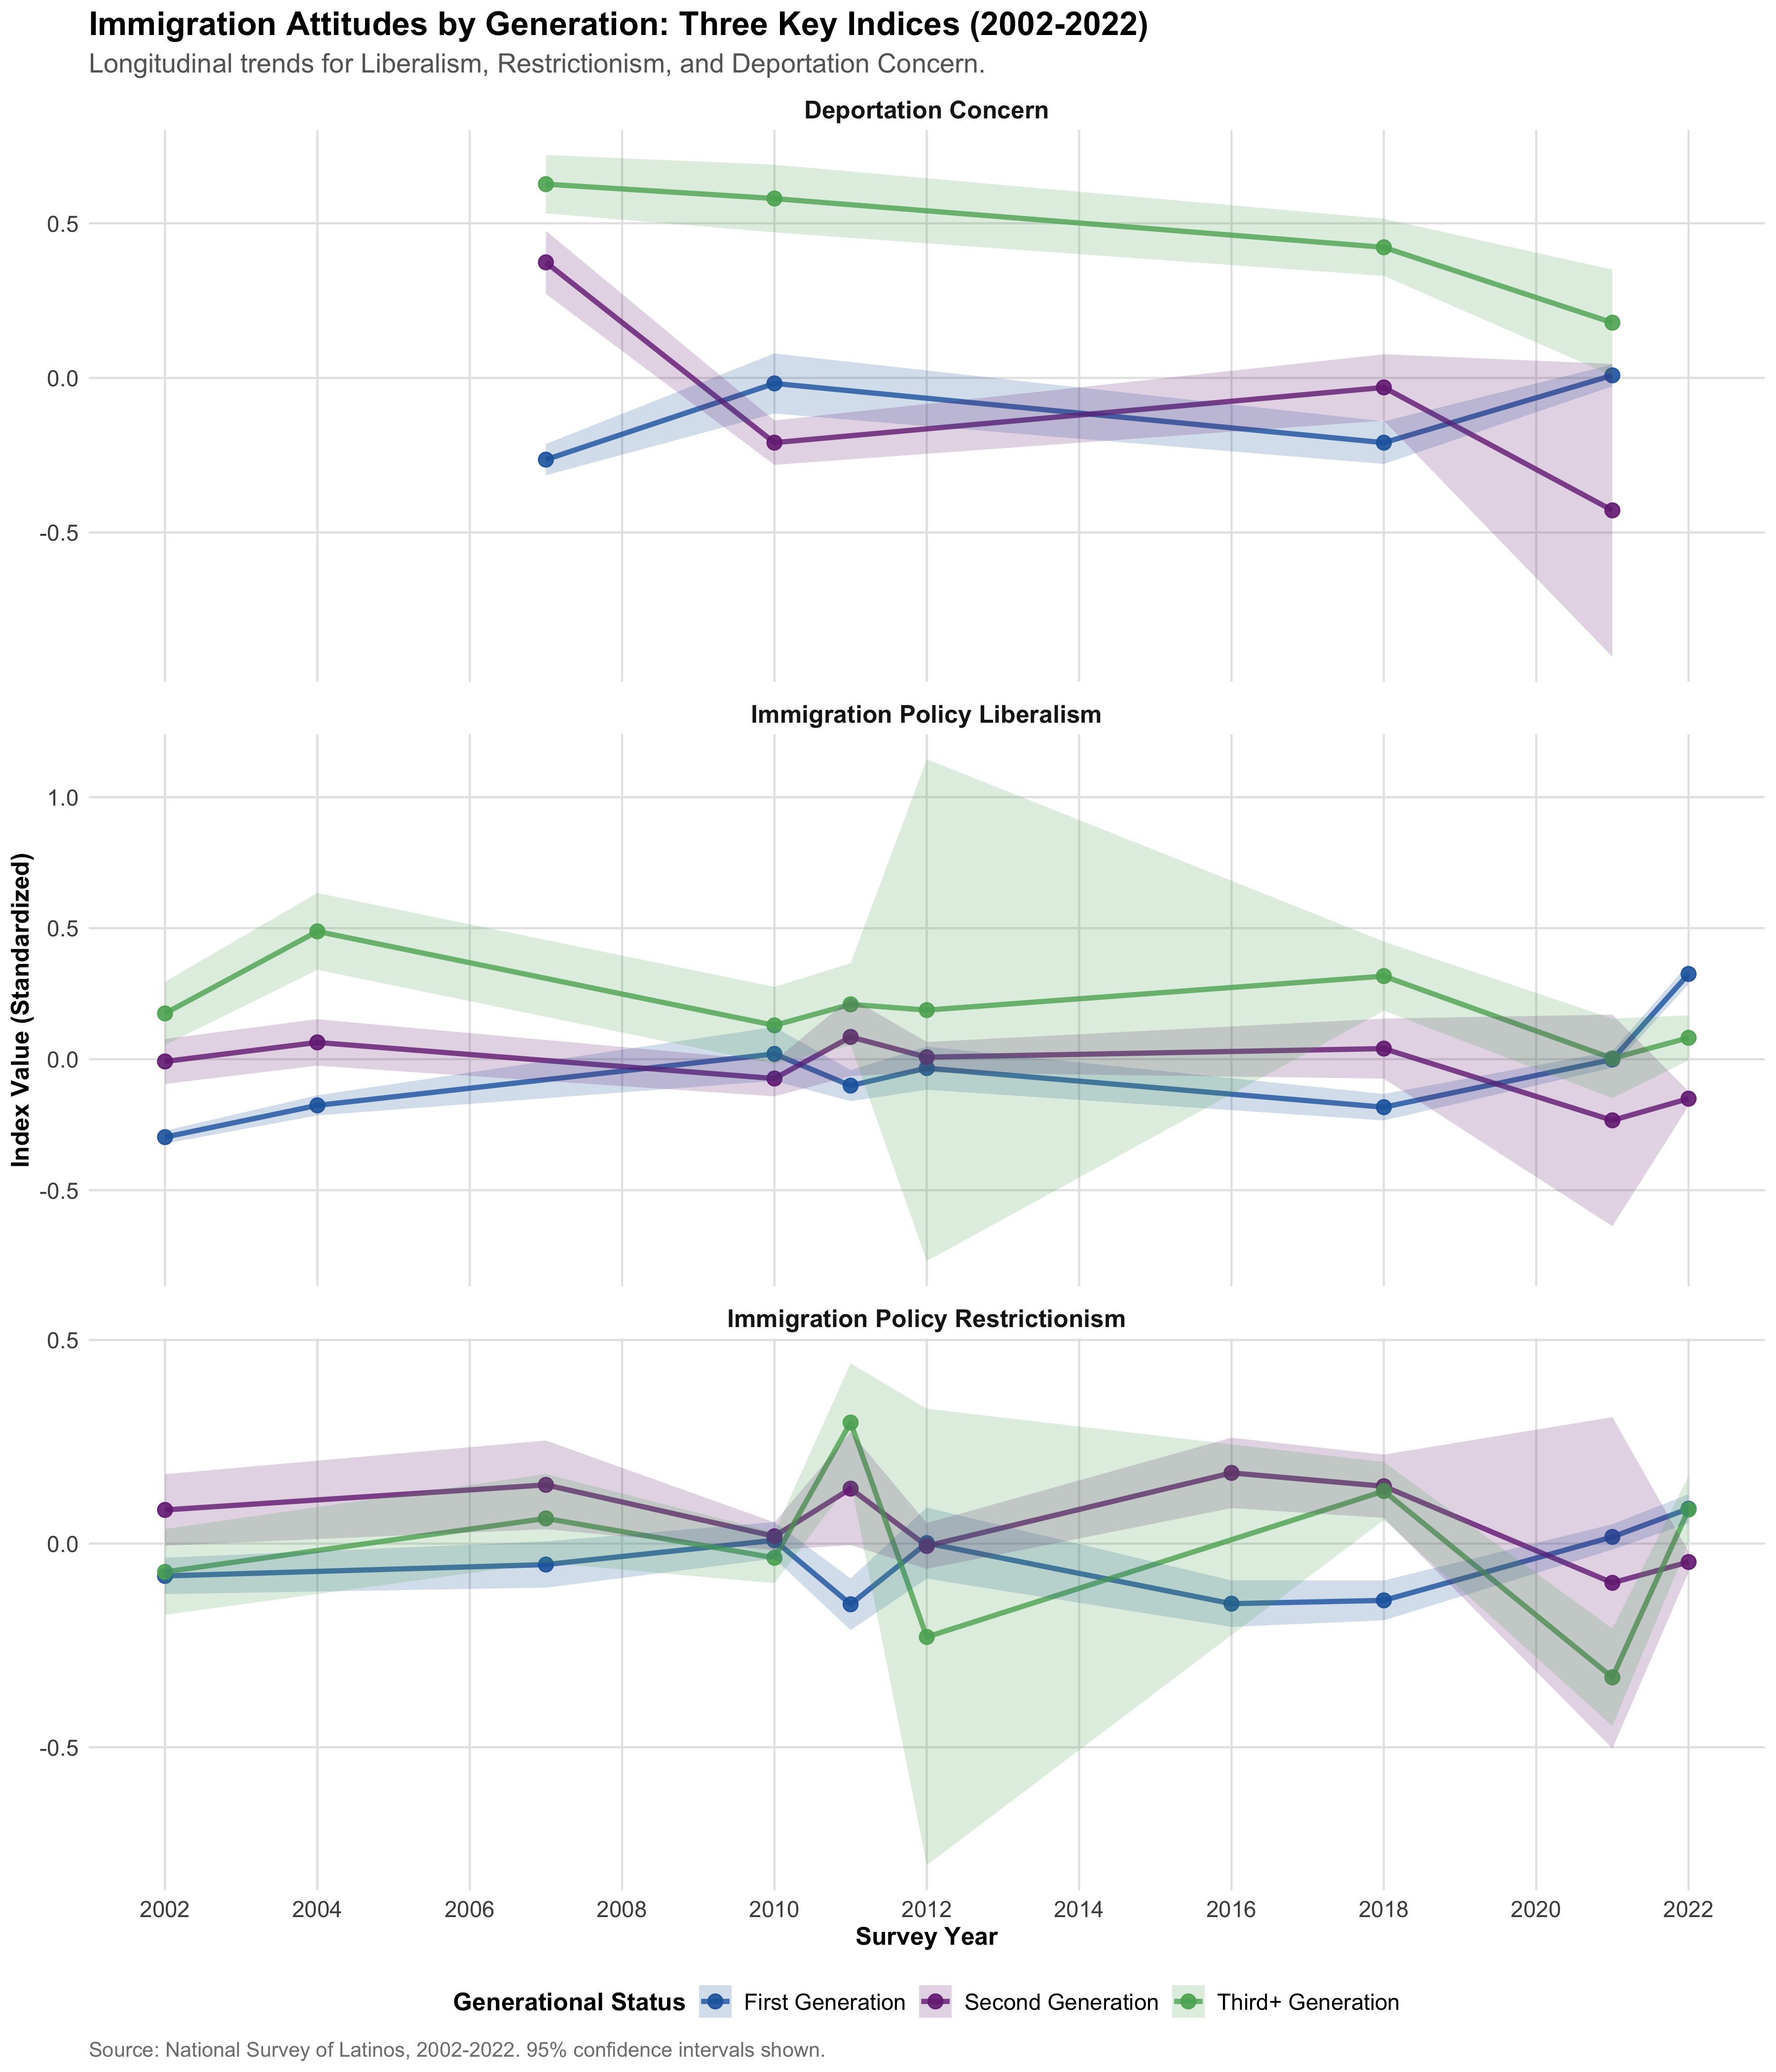
\includegraphics[width=\textwidth]{../../outputs/CURRENT_2025_08_09_FIGURES_gold_standard/three_indices_by_generation_2002_2022.png}
    \caption{Immigration attitudes by generation across three key thematic indices. This analysis reveals distinct generational patterns in liberalism, restrictionism, and deportation concern over the 20-year study period.}
    \label{fig:three_indices}
\end{figure}

\section{Trend Analysis}

\subsection{Overall Population Trends}

\begin{figure}[H]
    \centering
    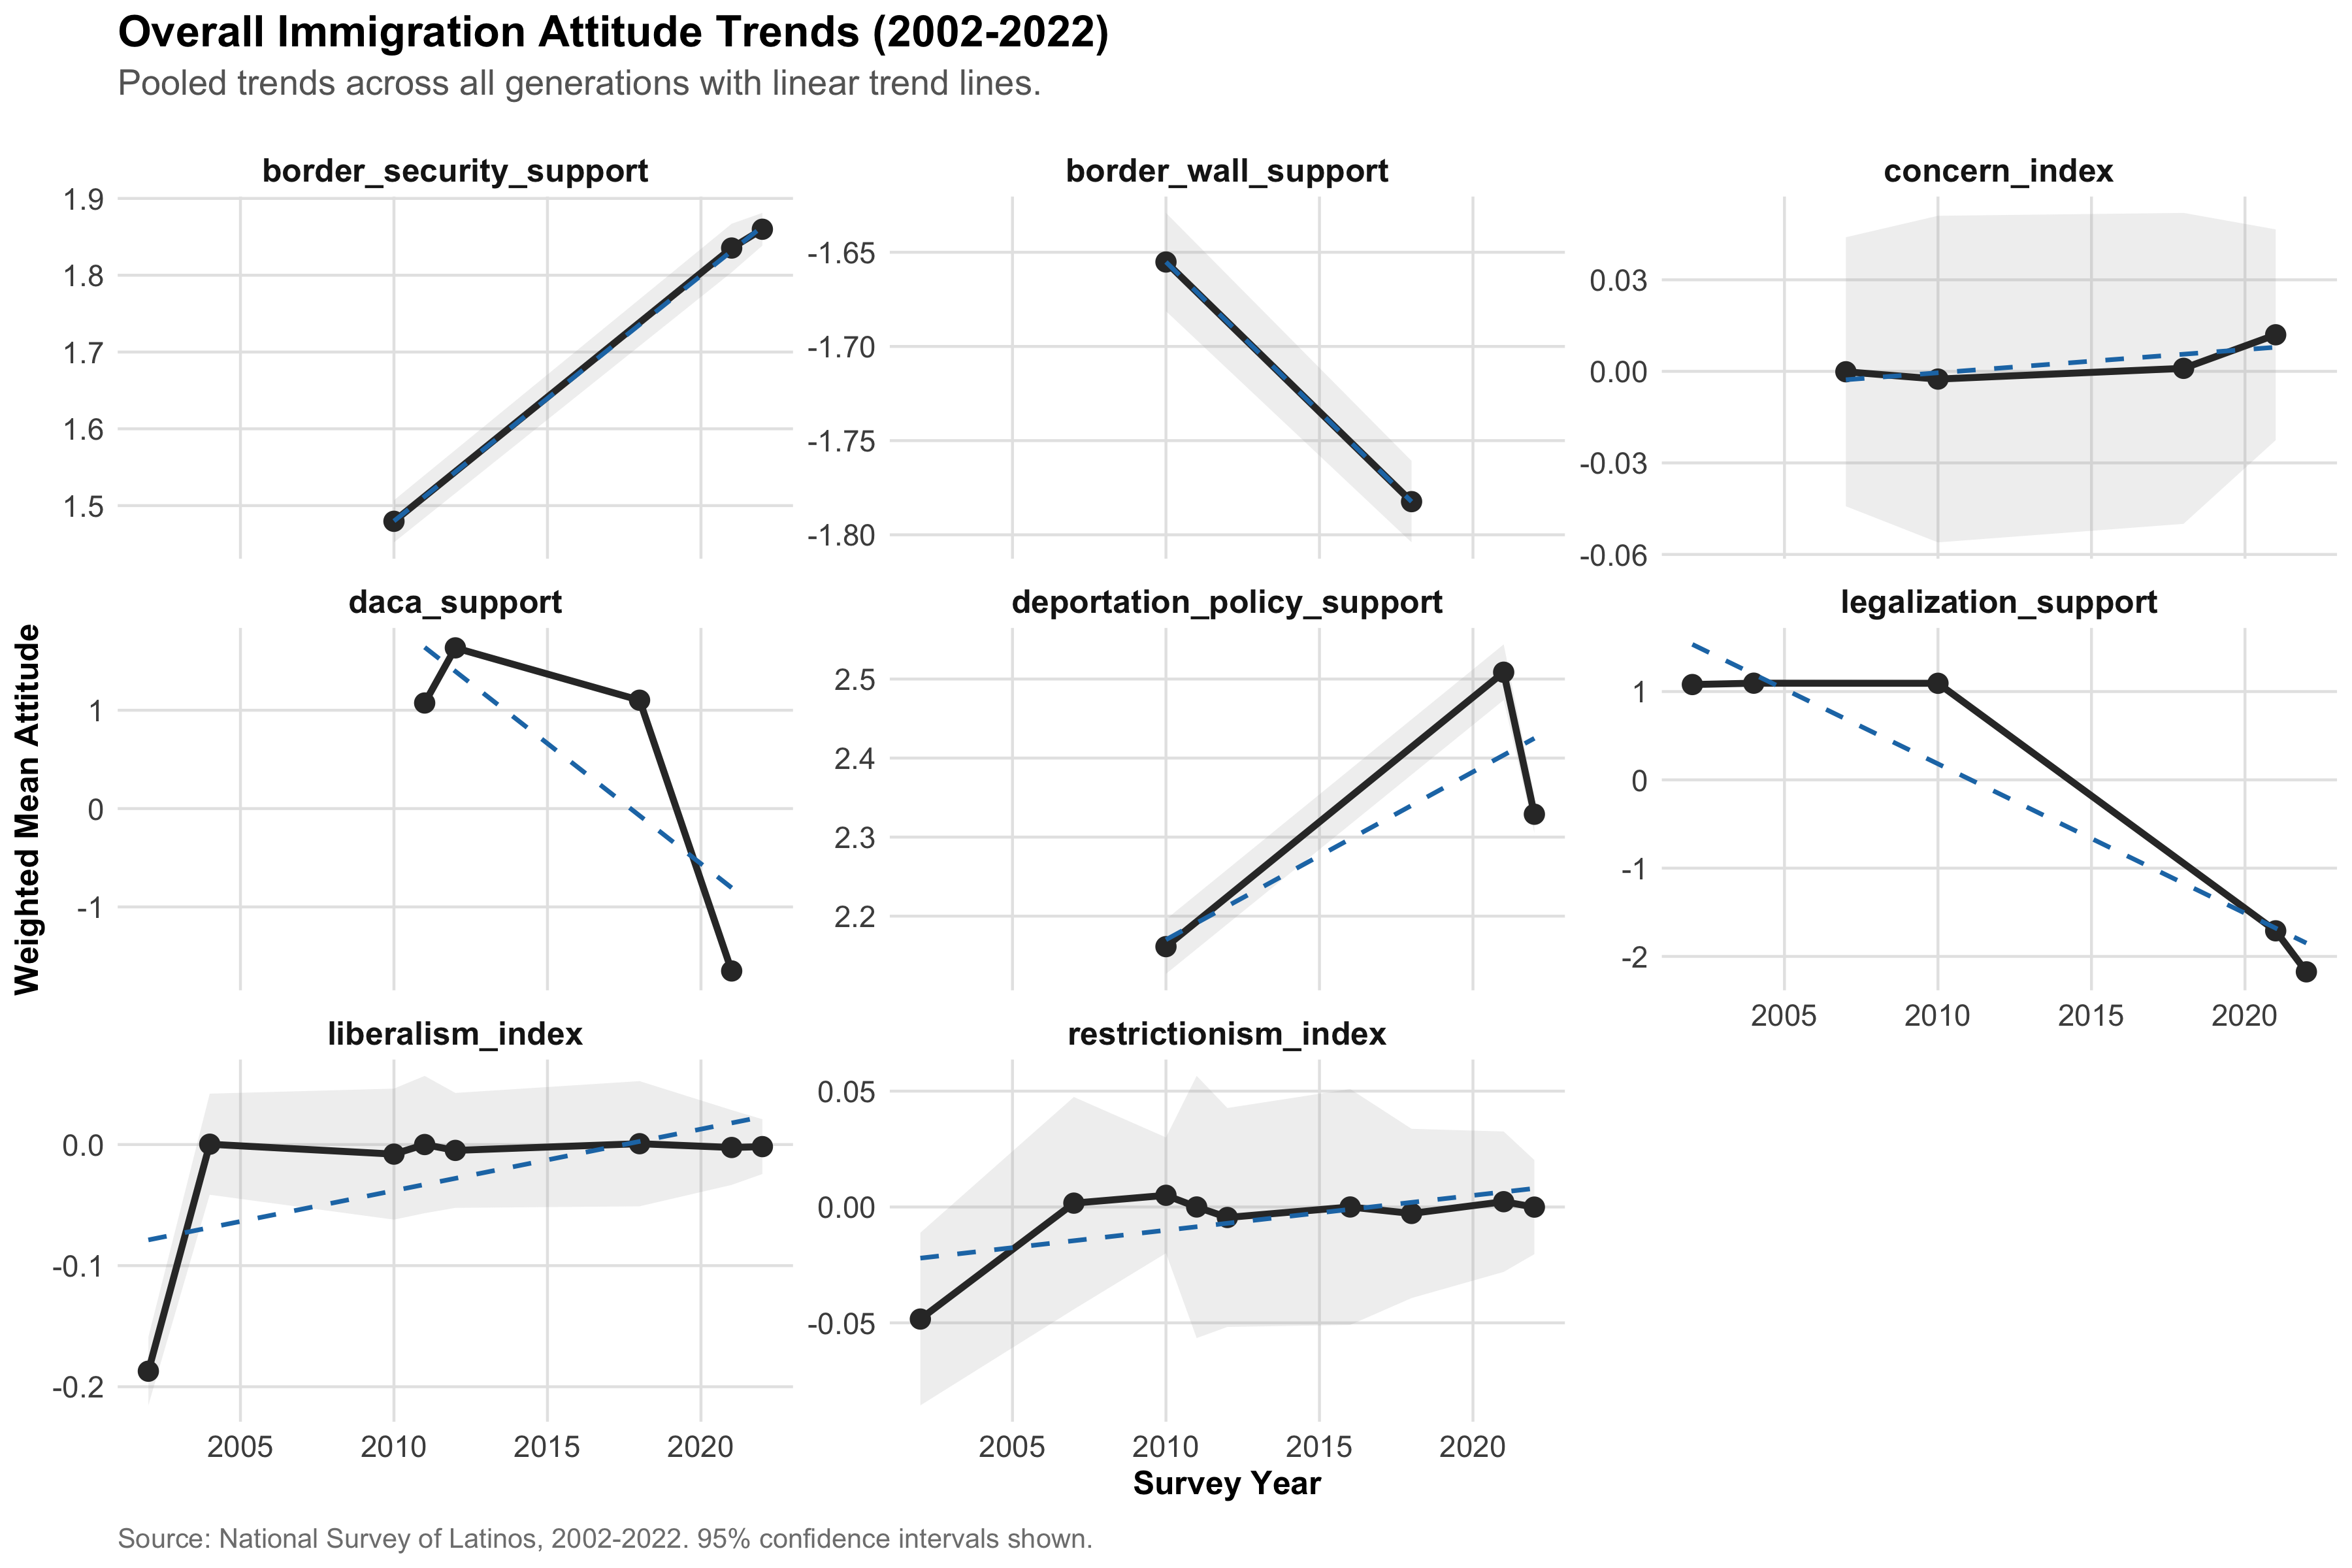
\includegraphics[width=\textwidth]{../../outputs/CURRENT_2025_08_09_FIGURES_gold_standard/overall_trends_2002_2022.png}
    \caption{Overall immigration attitude trends pooled across all generations, showing aggregate changes in attitudes over time with linear trend lines.}
    \label{fig:overall_trends}
\end{figure}

\subsection{Generation-Stratified Trends}

\begin{figure}[H]
    \centering
    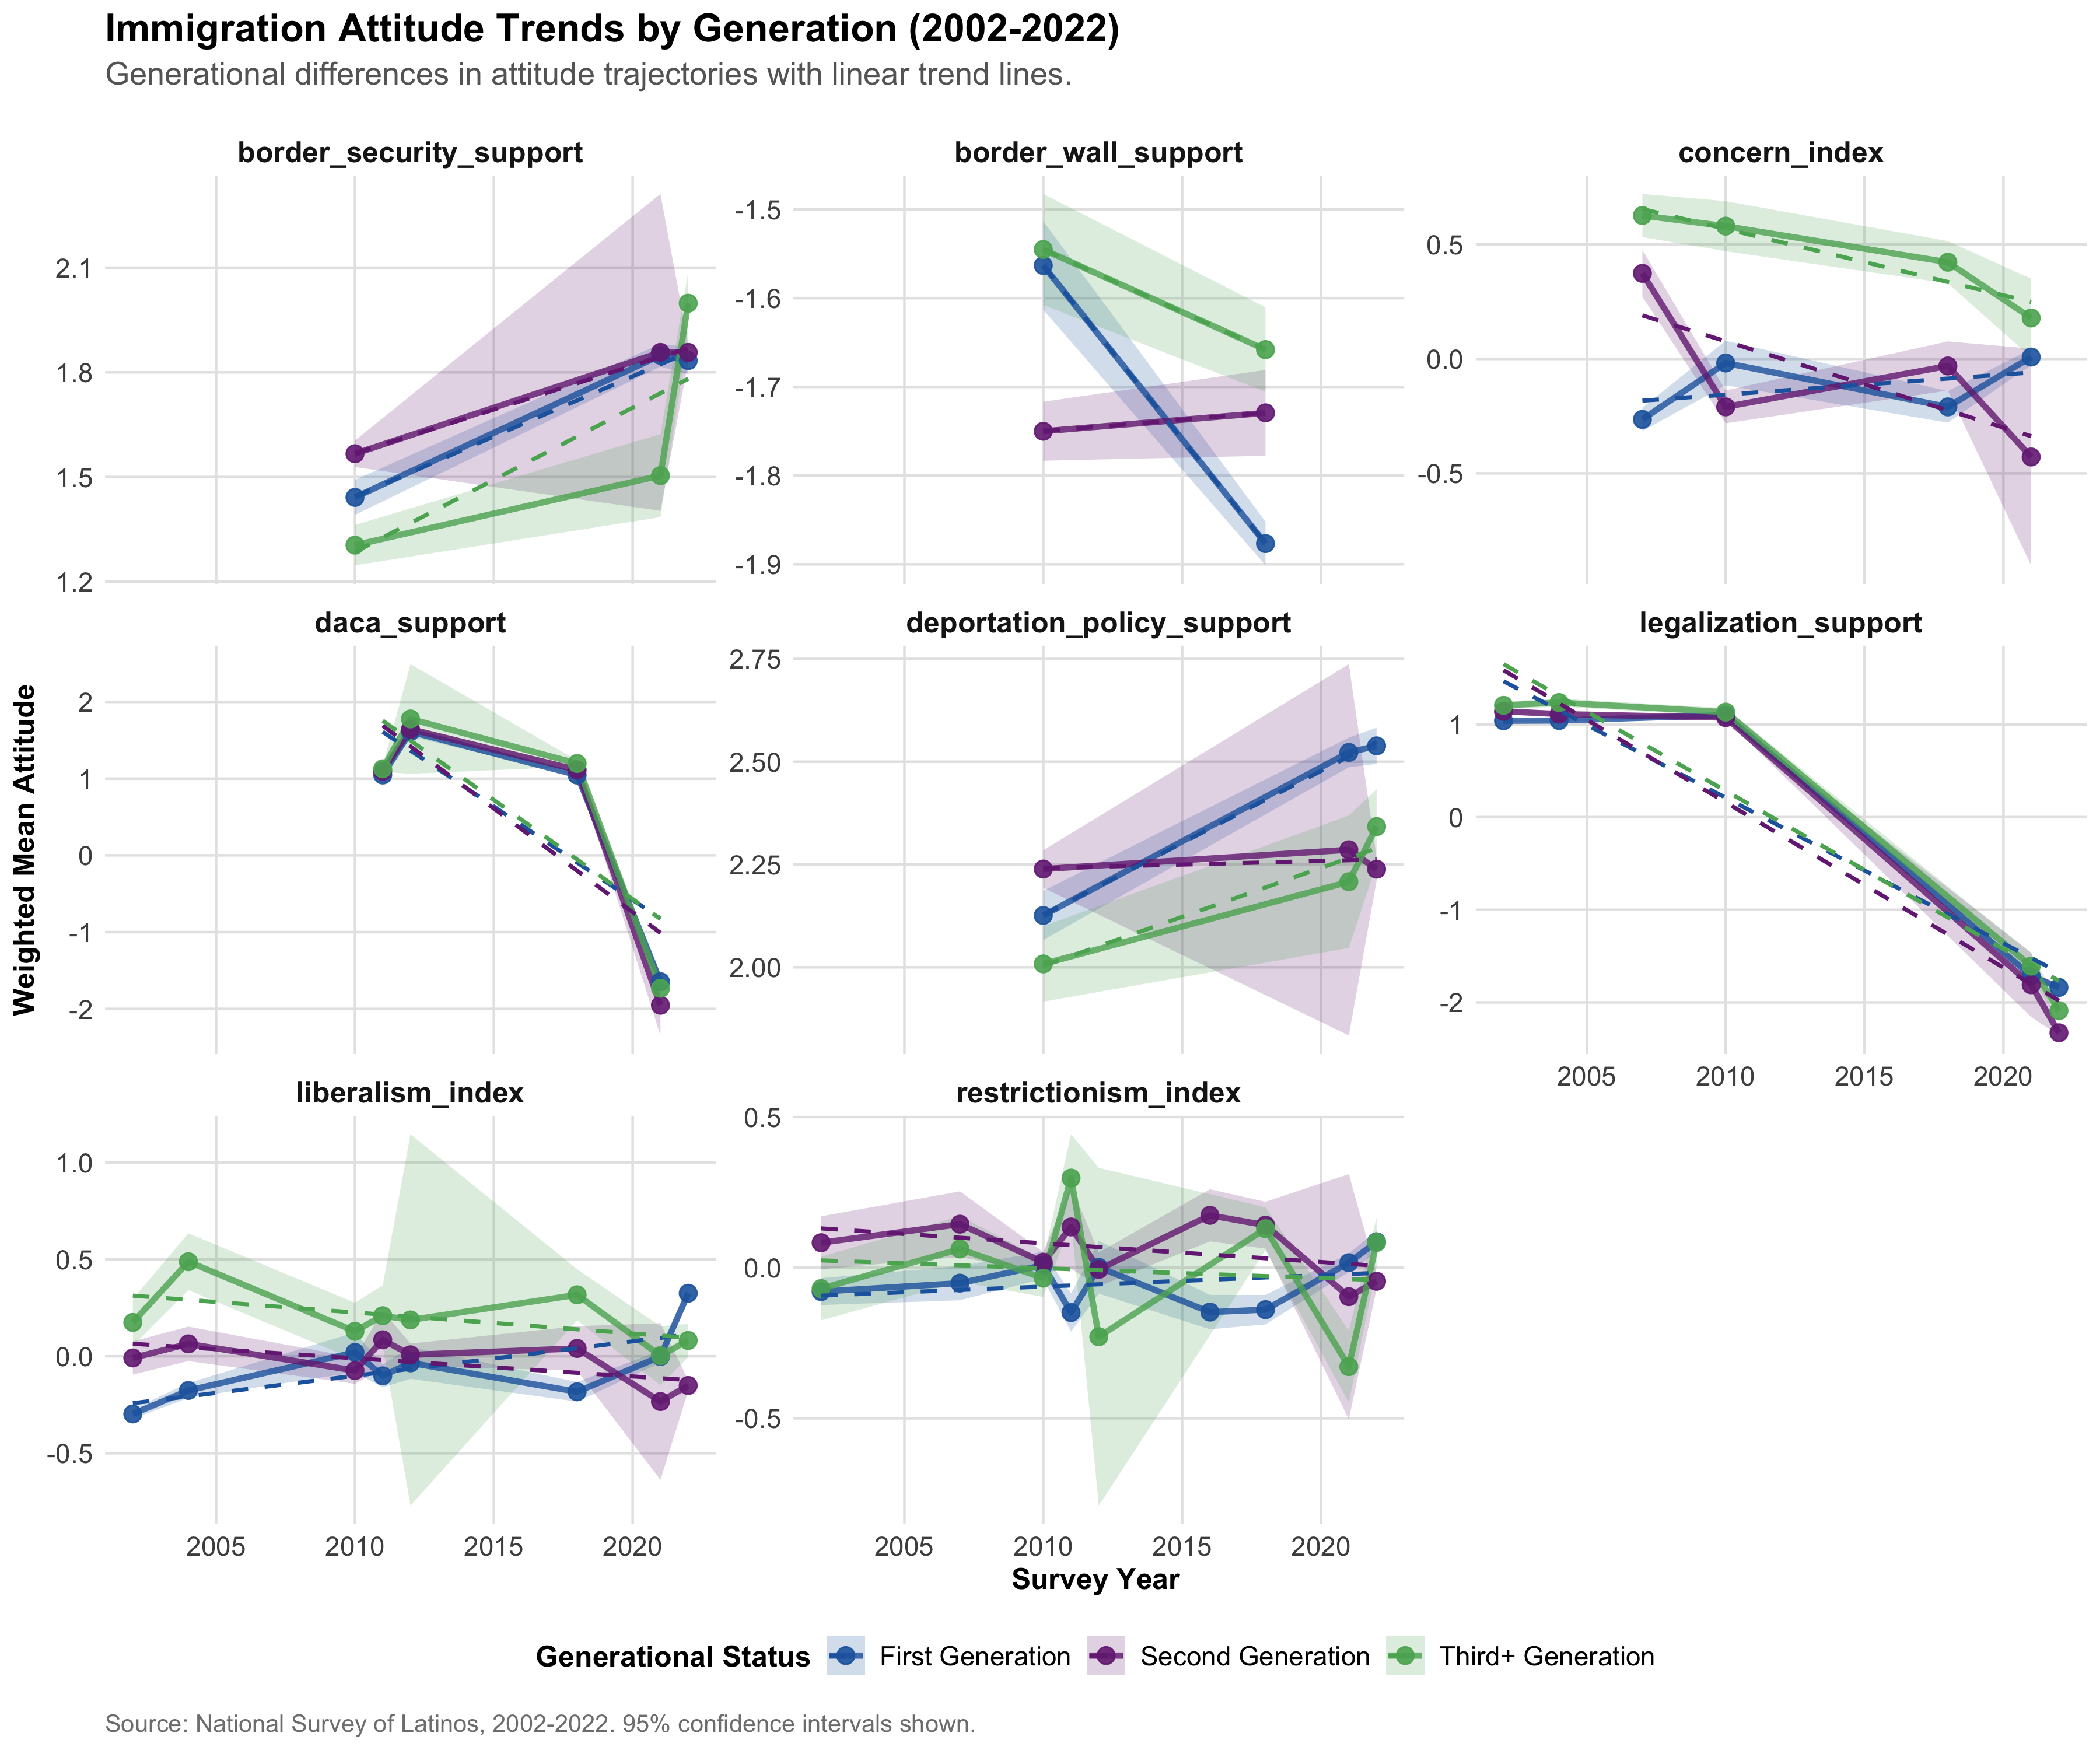
\includegraphics[width=\textwidth]{../../outputs/CURRENT_2025_08_09_FIGURES_gold_standard/generation_trends_2002_2022.png}
    \caption{Generation-specific immigration attitude trends revealing distinct trajectories for first, second, and third-plus generation respondents.}
    \label{fig:generation_trends}
\end{figure}

\section{Cross-Sectional Analysis}

\begin{figure}[H]
    \centering
    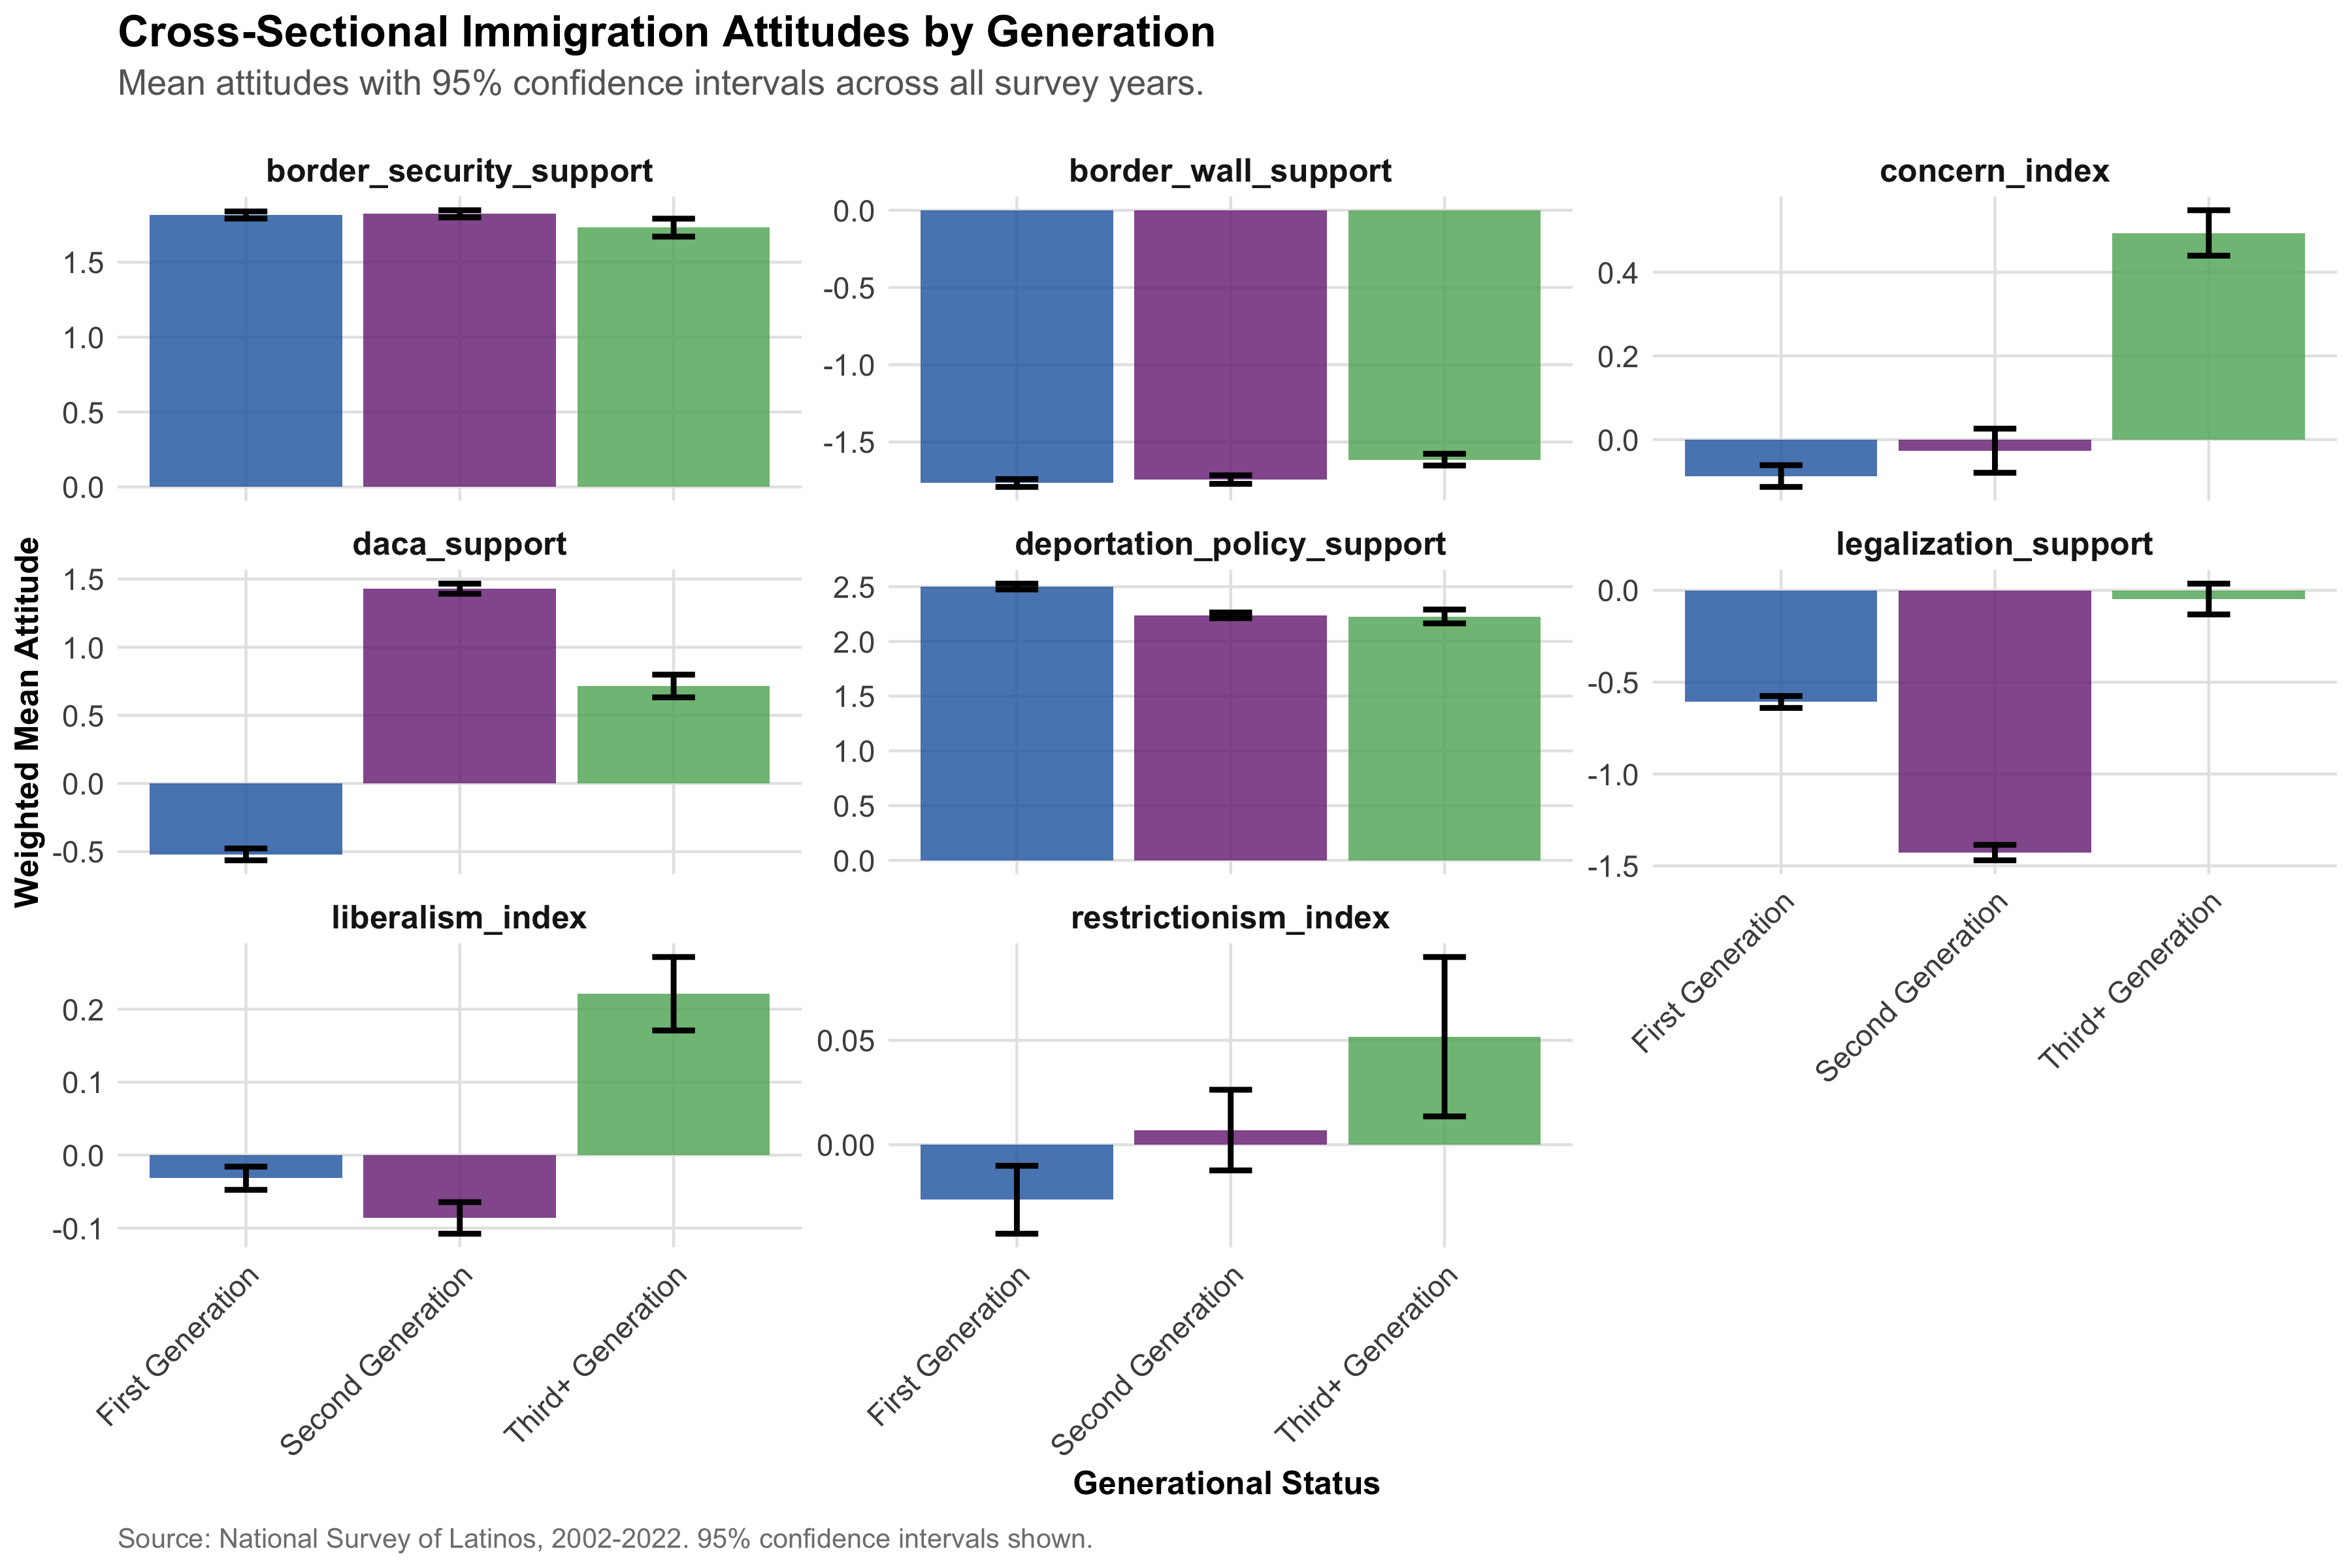
\includegraphics[width=\textwidth]{../../outputs/CURRENT_2025_08_09_FIGURES_gold_standard/cross_sectional_means.png}
    \caption{Cross-sectional comparison of immigration attitudes by generation, showing mean differences with 95\% confidence intervals.}
    \label{fig:cross_sectional}
\end{figure}

\section{Data Quality and Coverage}

\subsection{Data Coverage Matrix}

\begin{figure}[H]
    \centering
    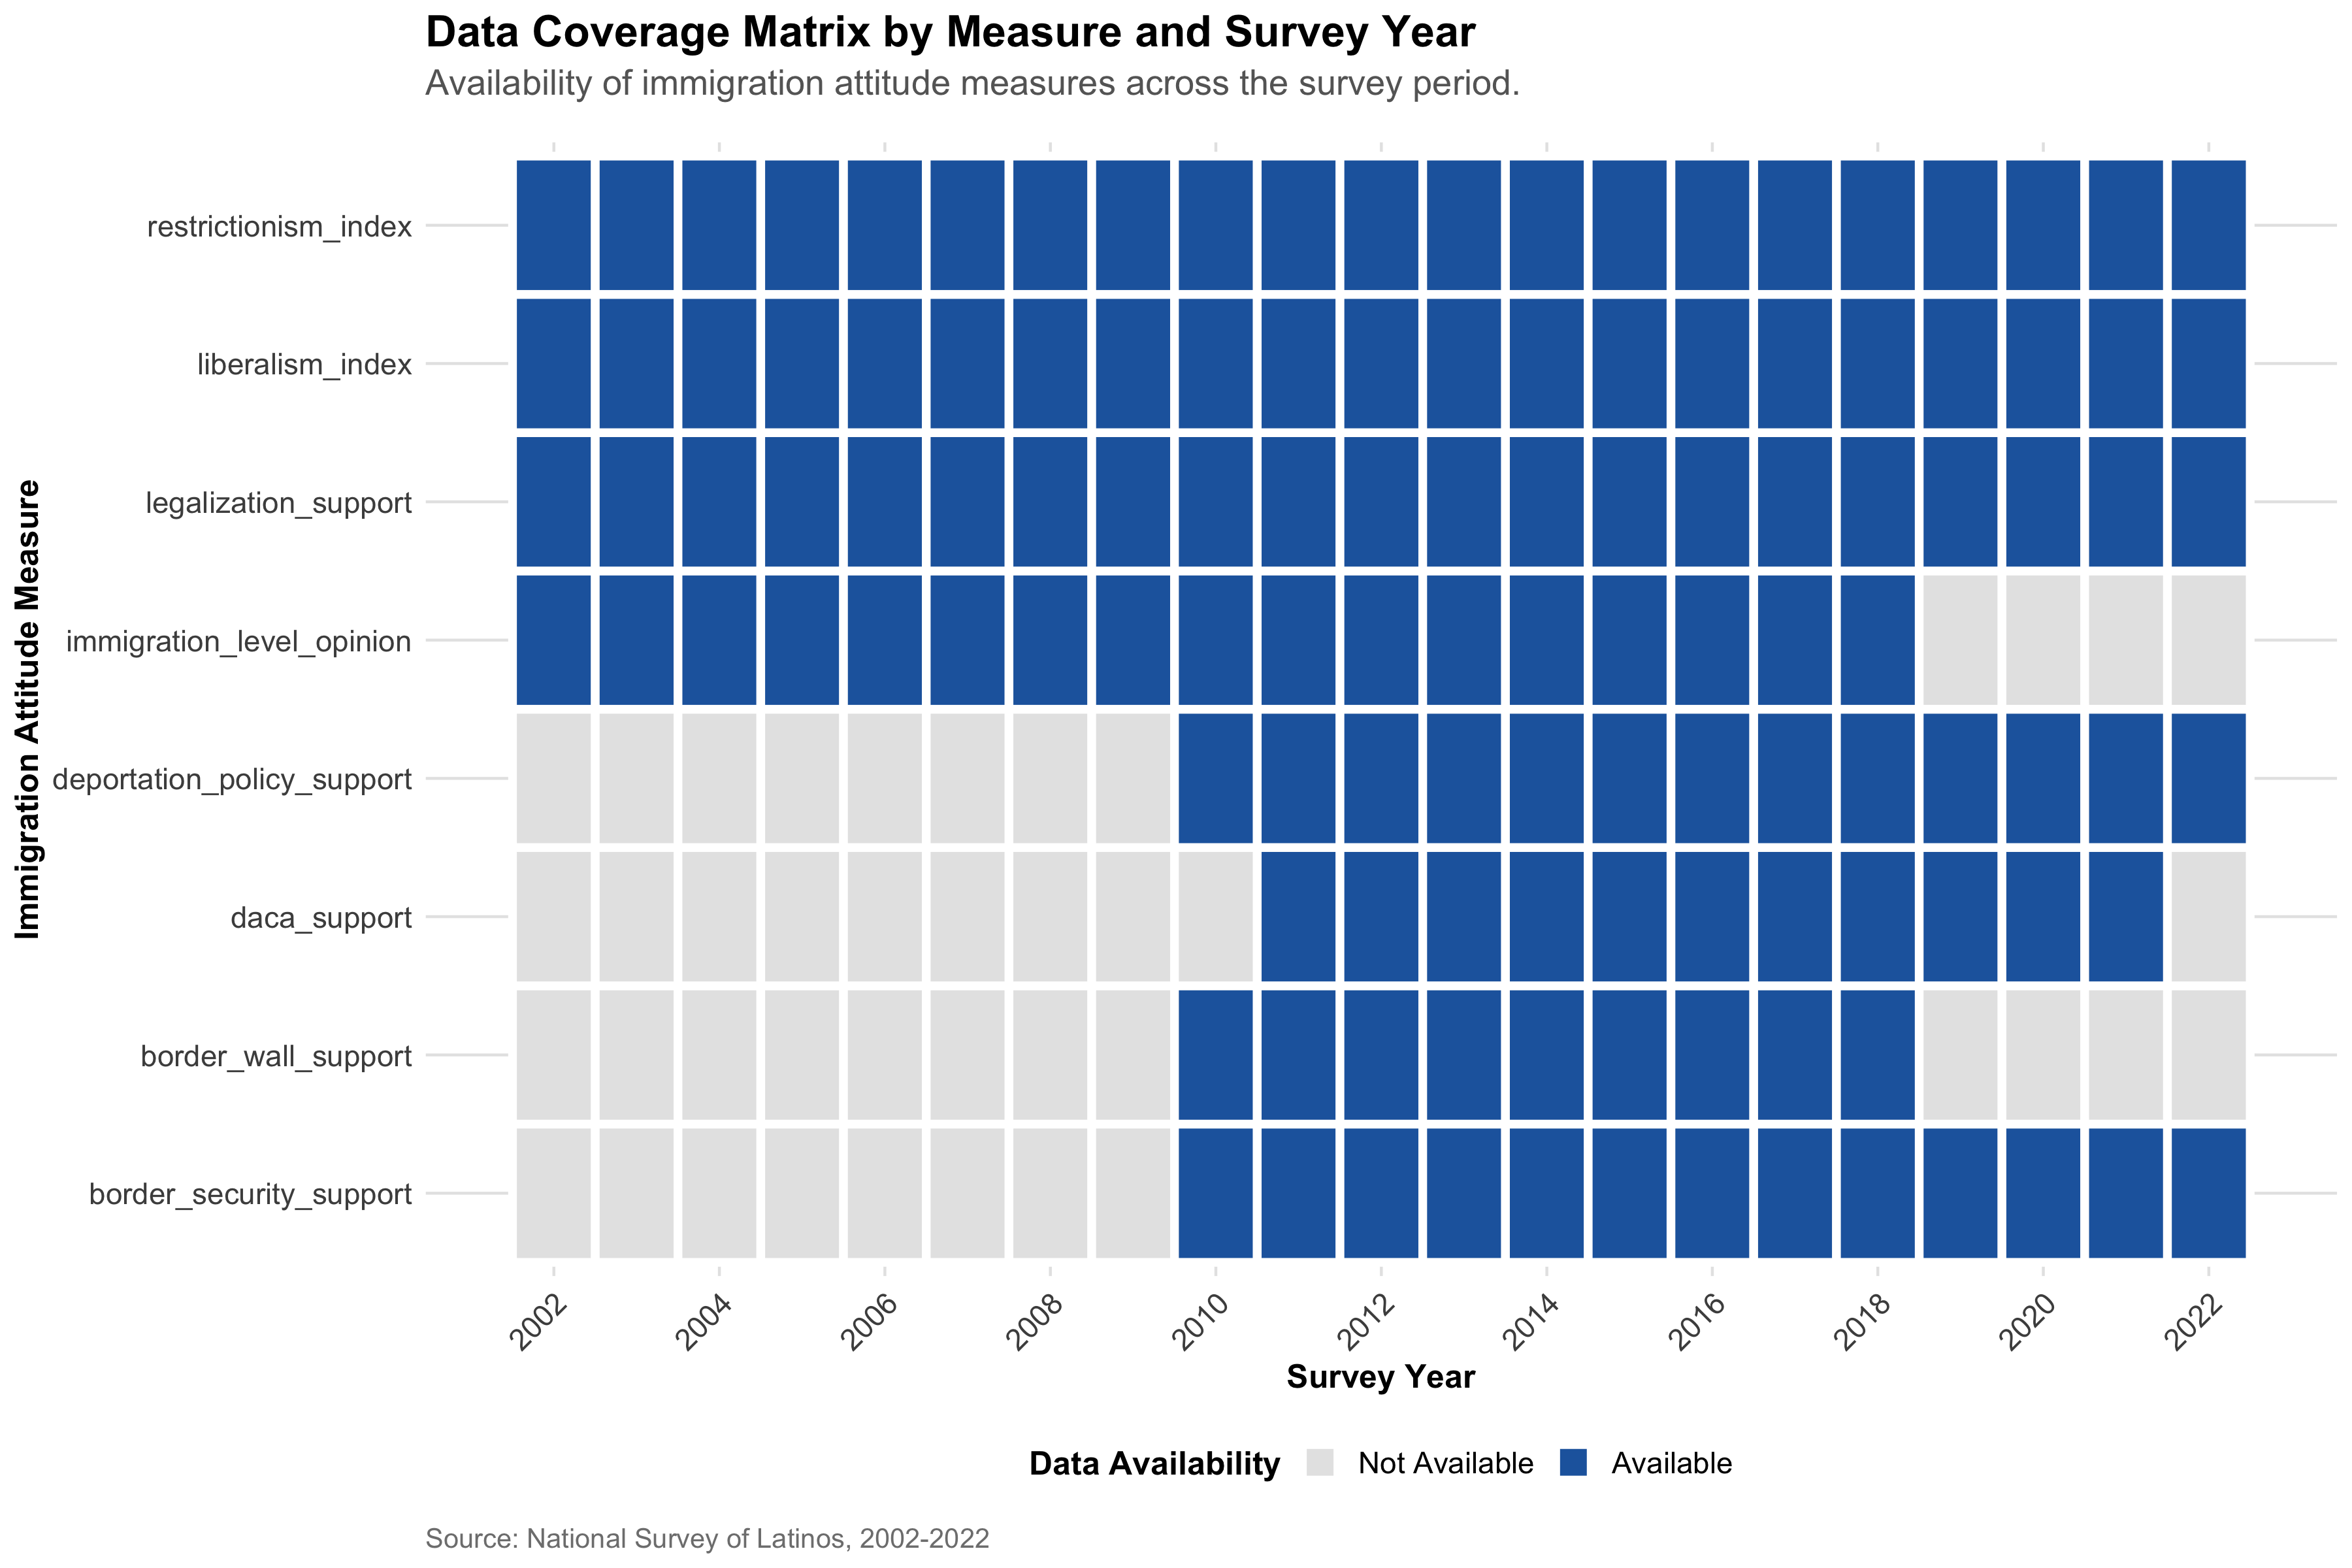
\includegraphics[width=\textwidth]{../../outputs/CURRENT_2025_08_09_FIGURES_gold_standard/data_coverage_matrix.png}
    \caption{Data availability matrix showing which immigration attitude measures are available across survey years, informing interpretation of trend analyses.}
    \label{fig:coverage}
\end{figure}

\subsection{Sample Composition}

\begin{figure}[H]
    \centering
    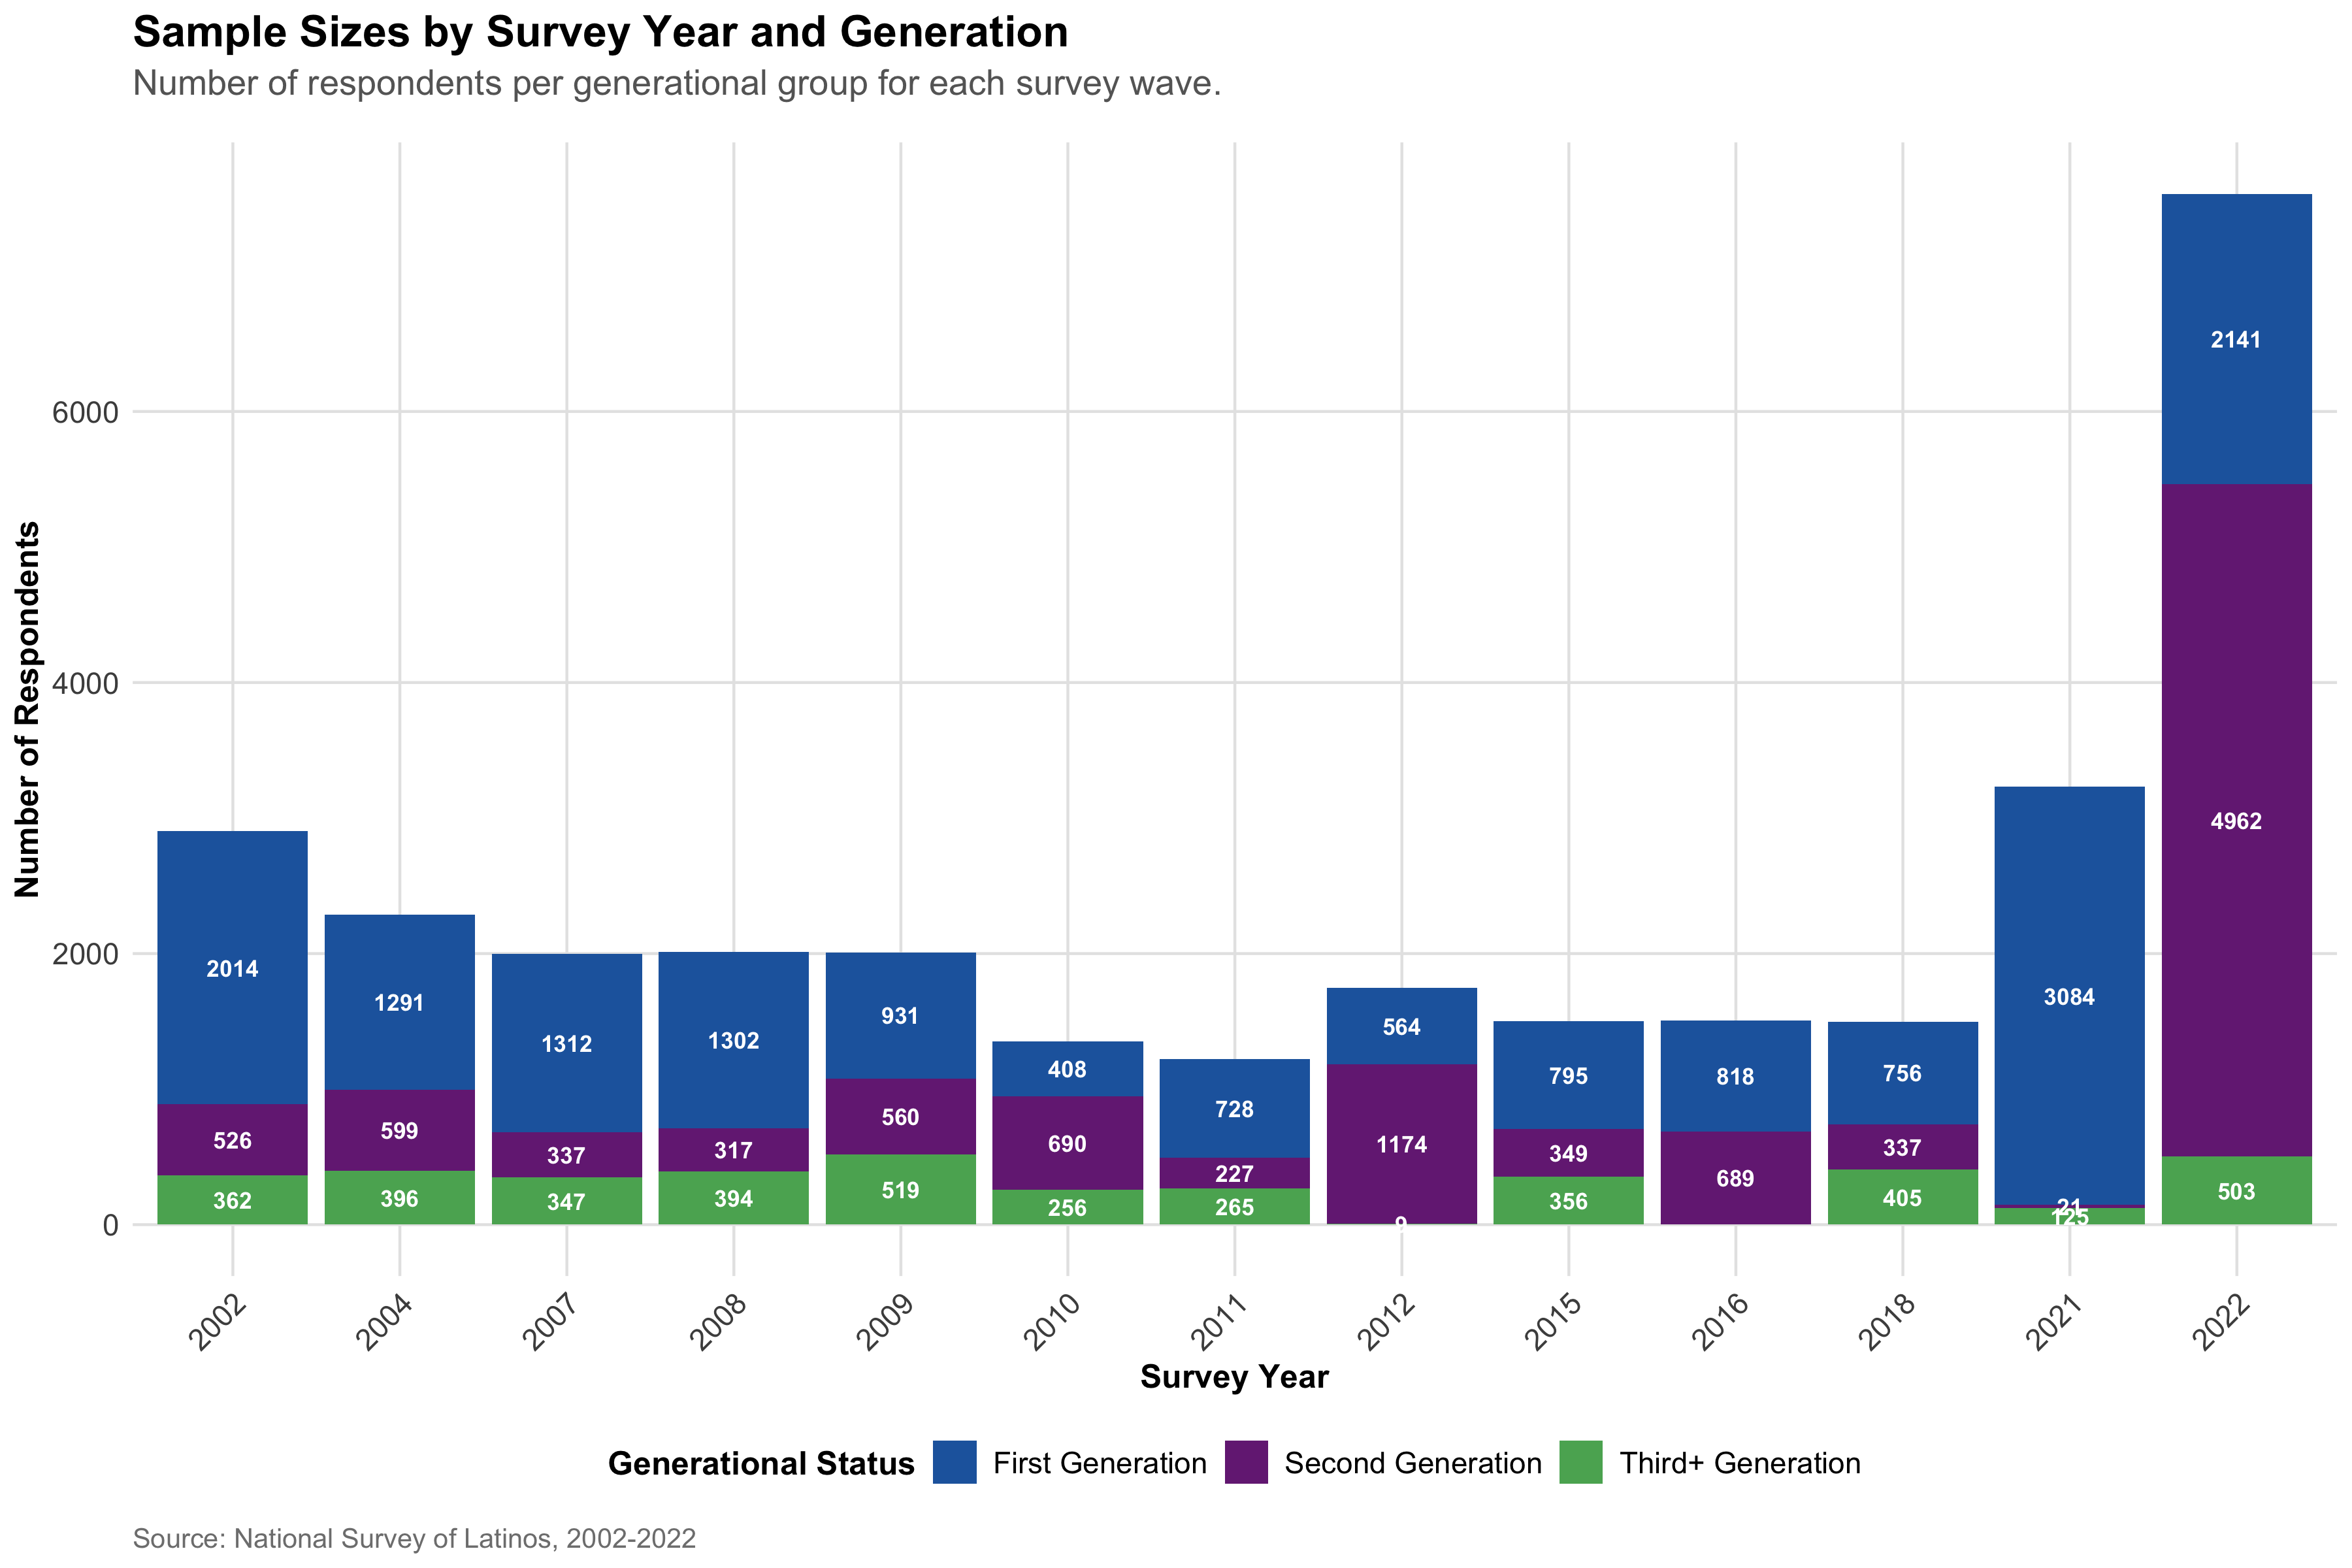
\includegraphics[width=\textwidth]{../../outputs/CURRENT_2025_08_09_FIGURES_gold_standard/sample_sizes_by_year.png}
    \caption{Sample sizes by survey year and generation, showing the number of respondents contributing to each analysis.}
    \label{fig:sample_sizes}
\end{figure}

\begin{figure}[H]
    \centering
    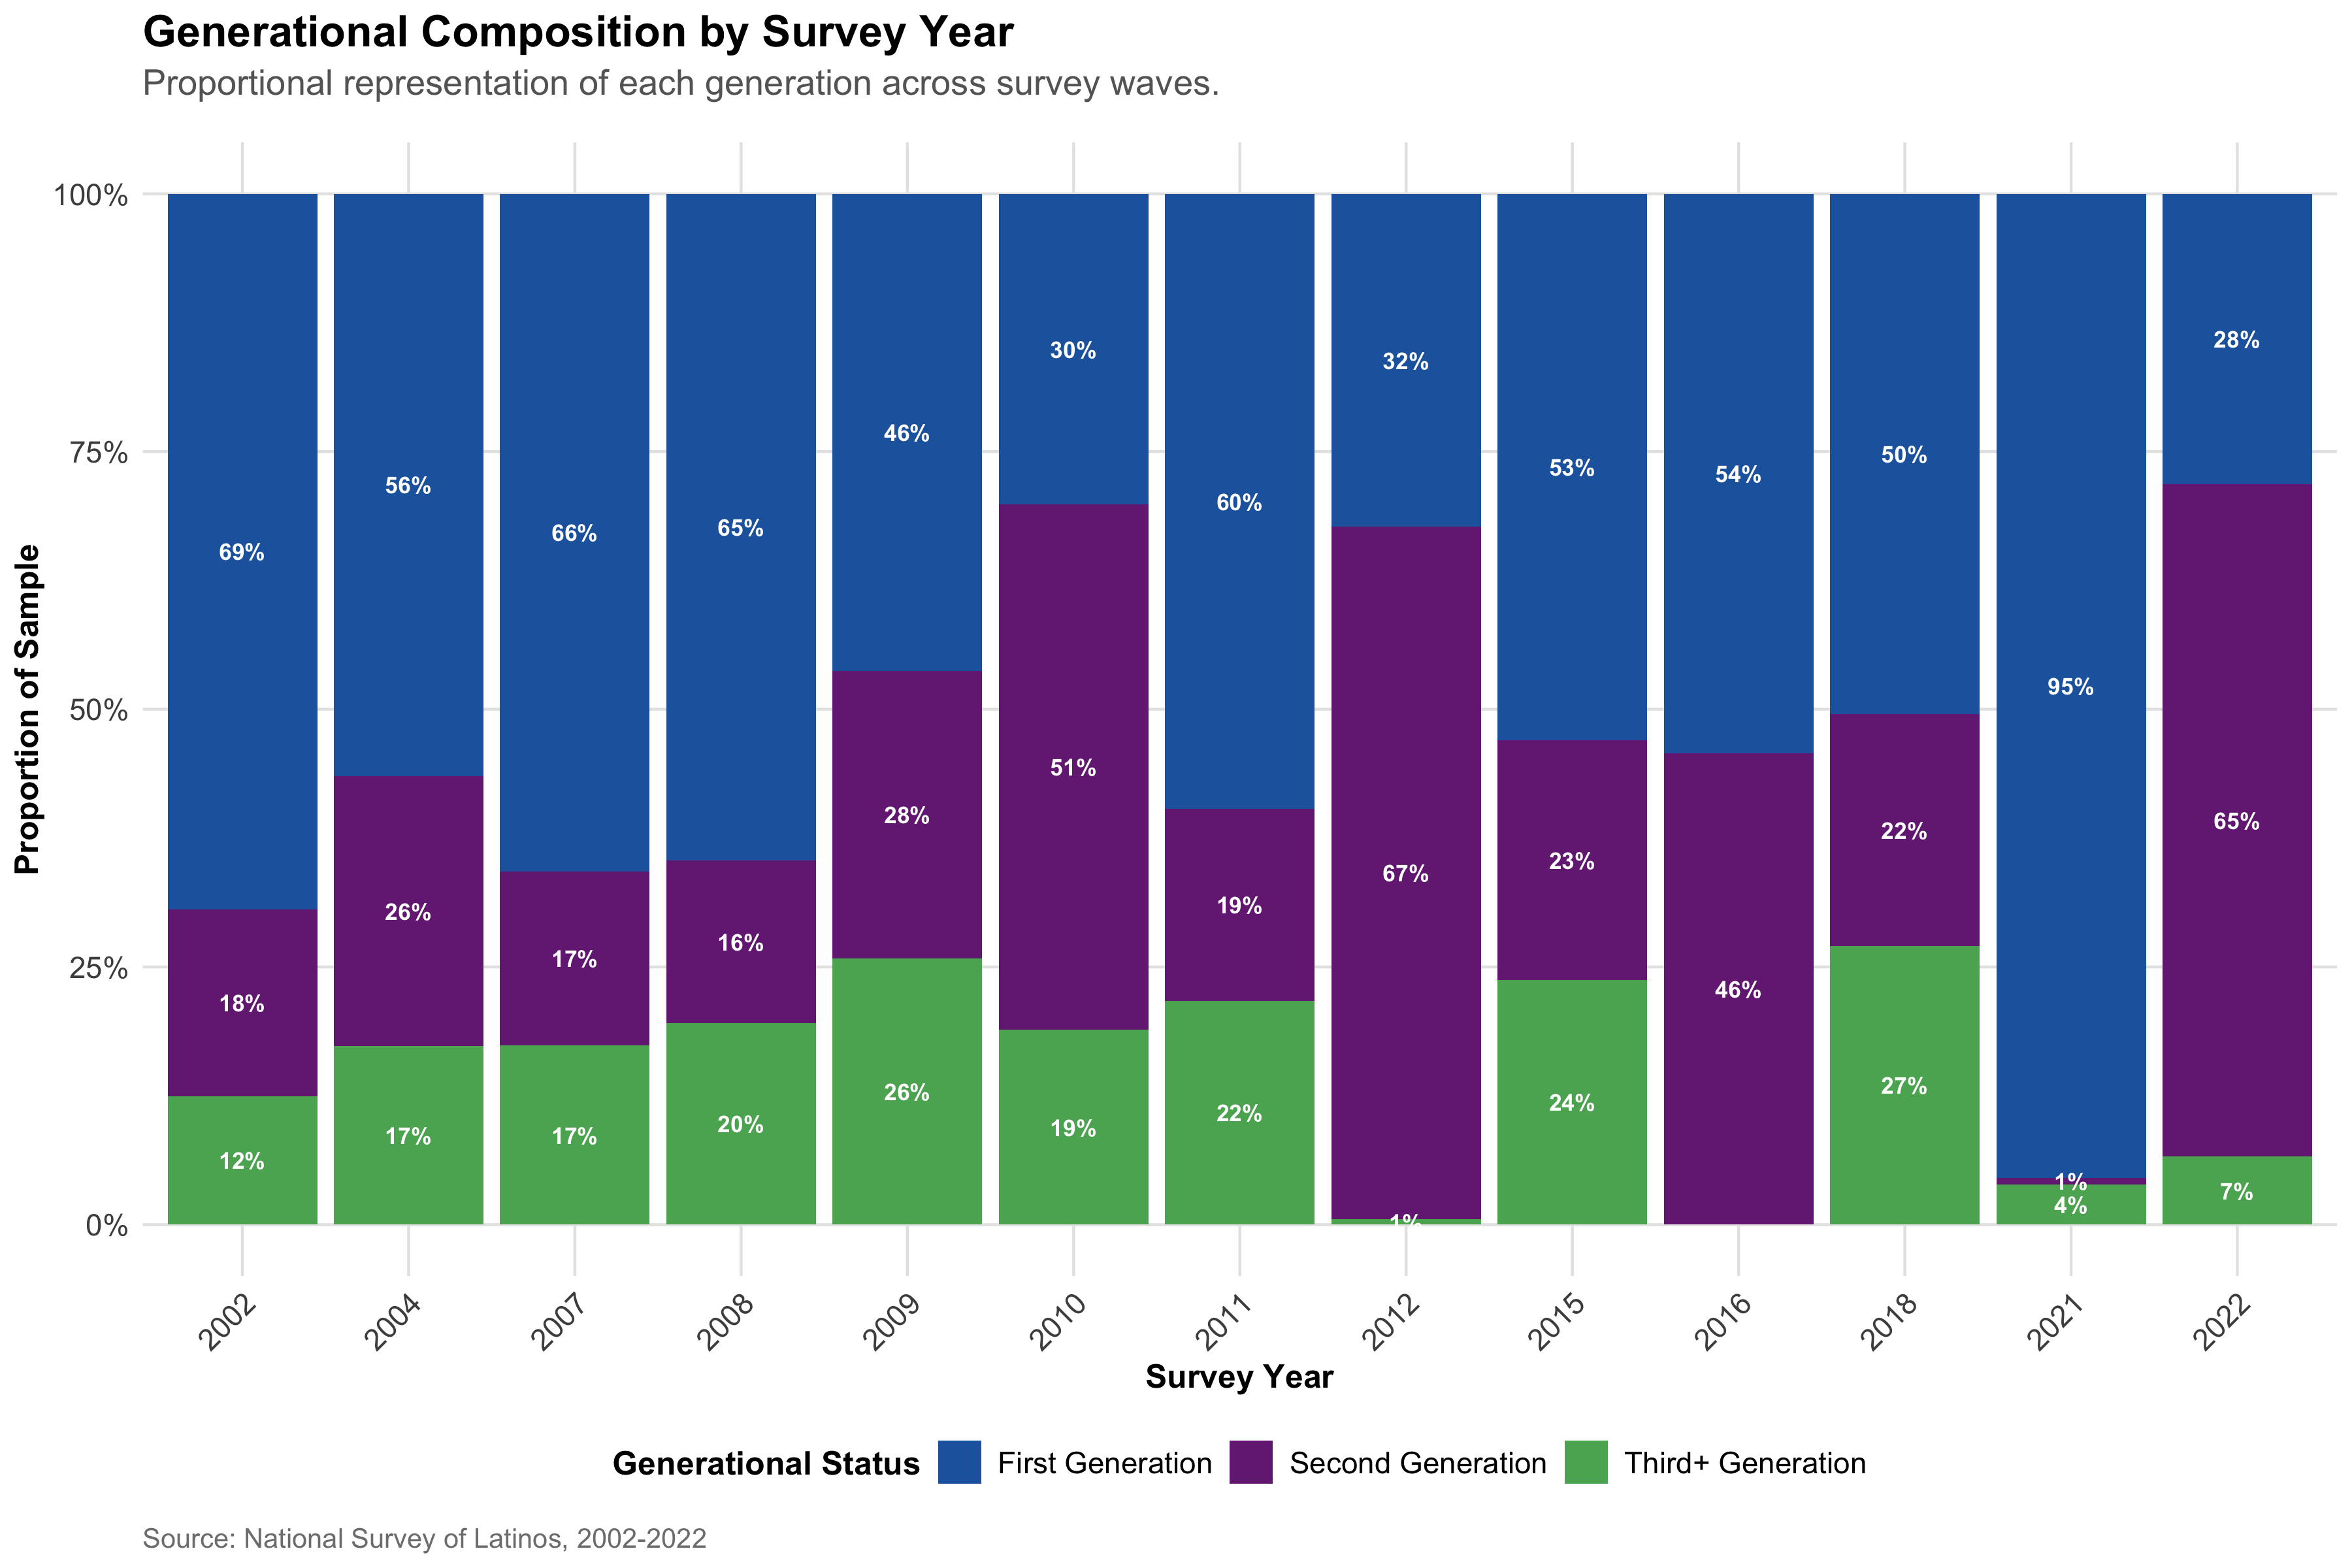
\includegraphics[width=\textwidth]{../../outputs/CURRENT_2025_08_09_FIGURES_gold_standard/generation_composition_by_year.png}
    \caption{Generational composition of the sample across survey years, illustrating changing demographic representation over time.}
    \label{fig:composition}
\end{figure}

\section{Statistical Analysis}

\subsection{Volatility Analysis}

\begin{figure}[H]
    \centering
    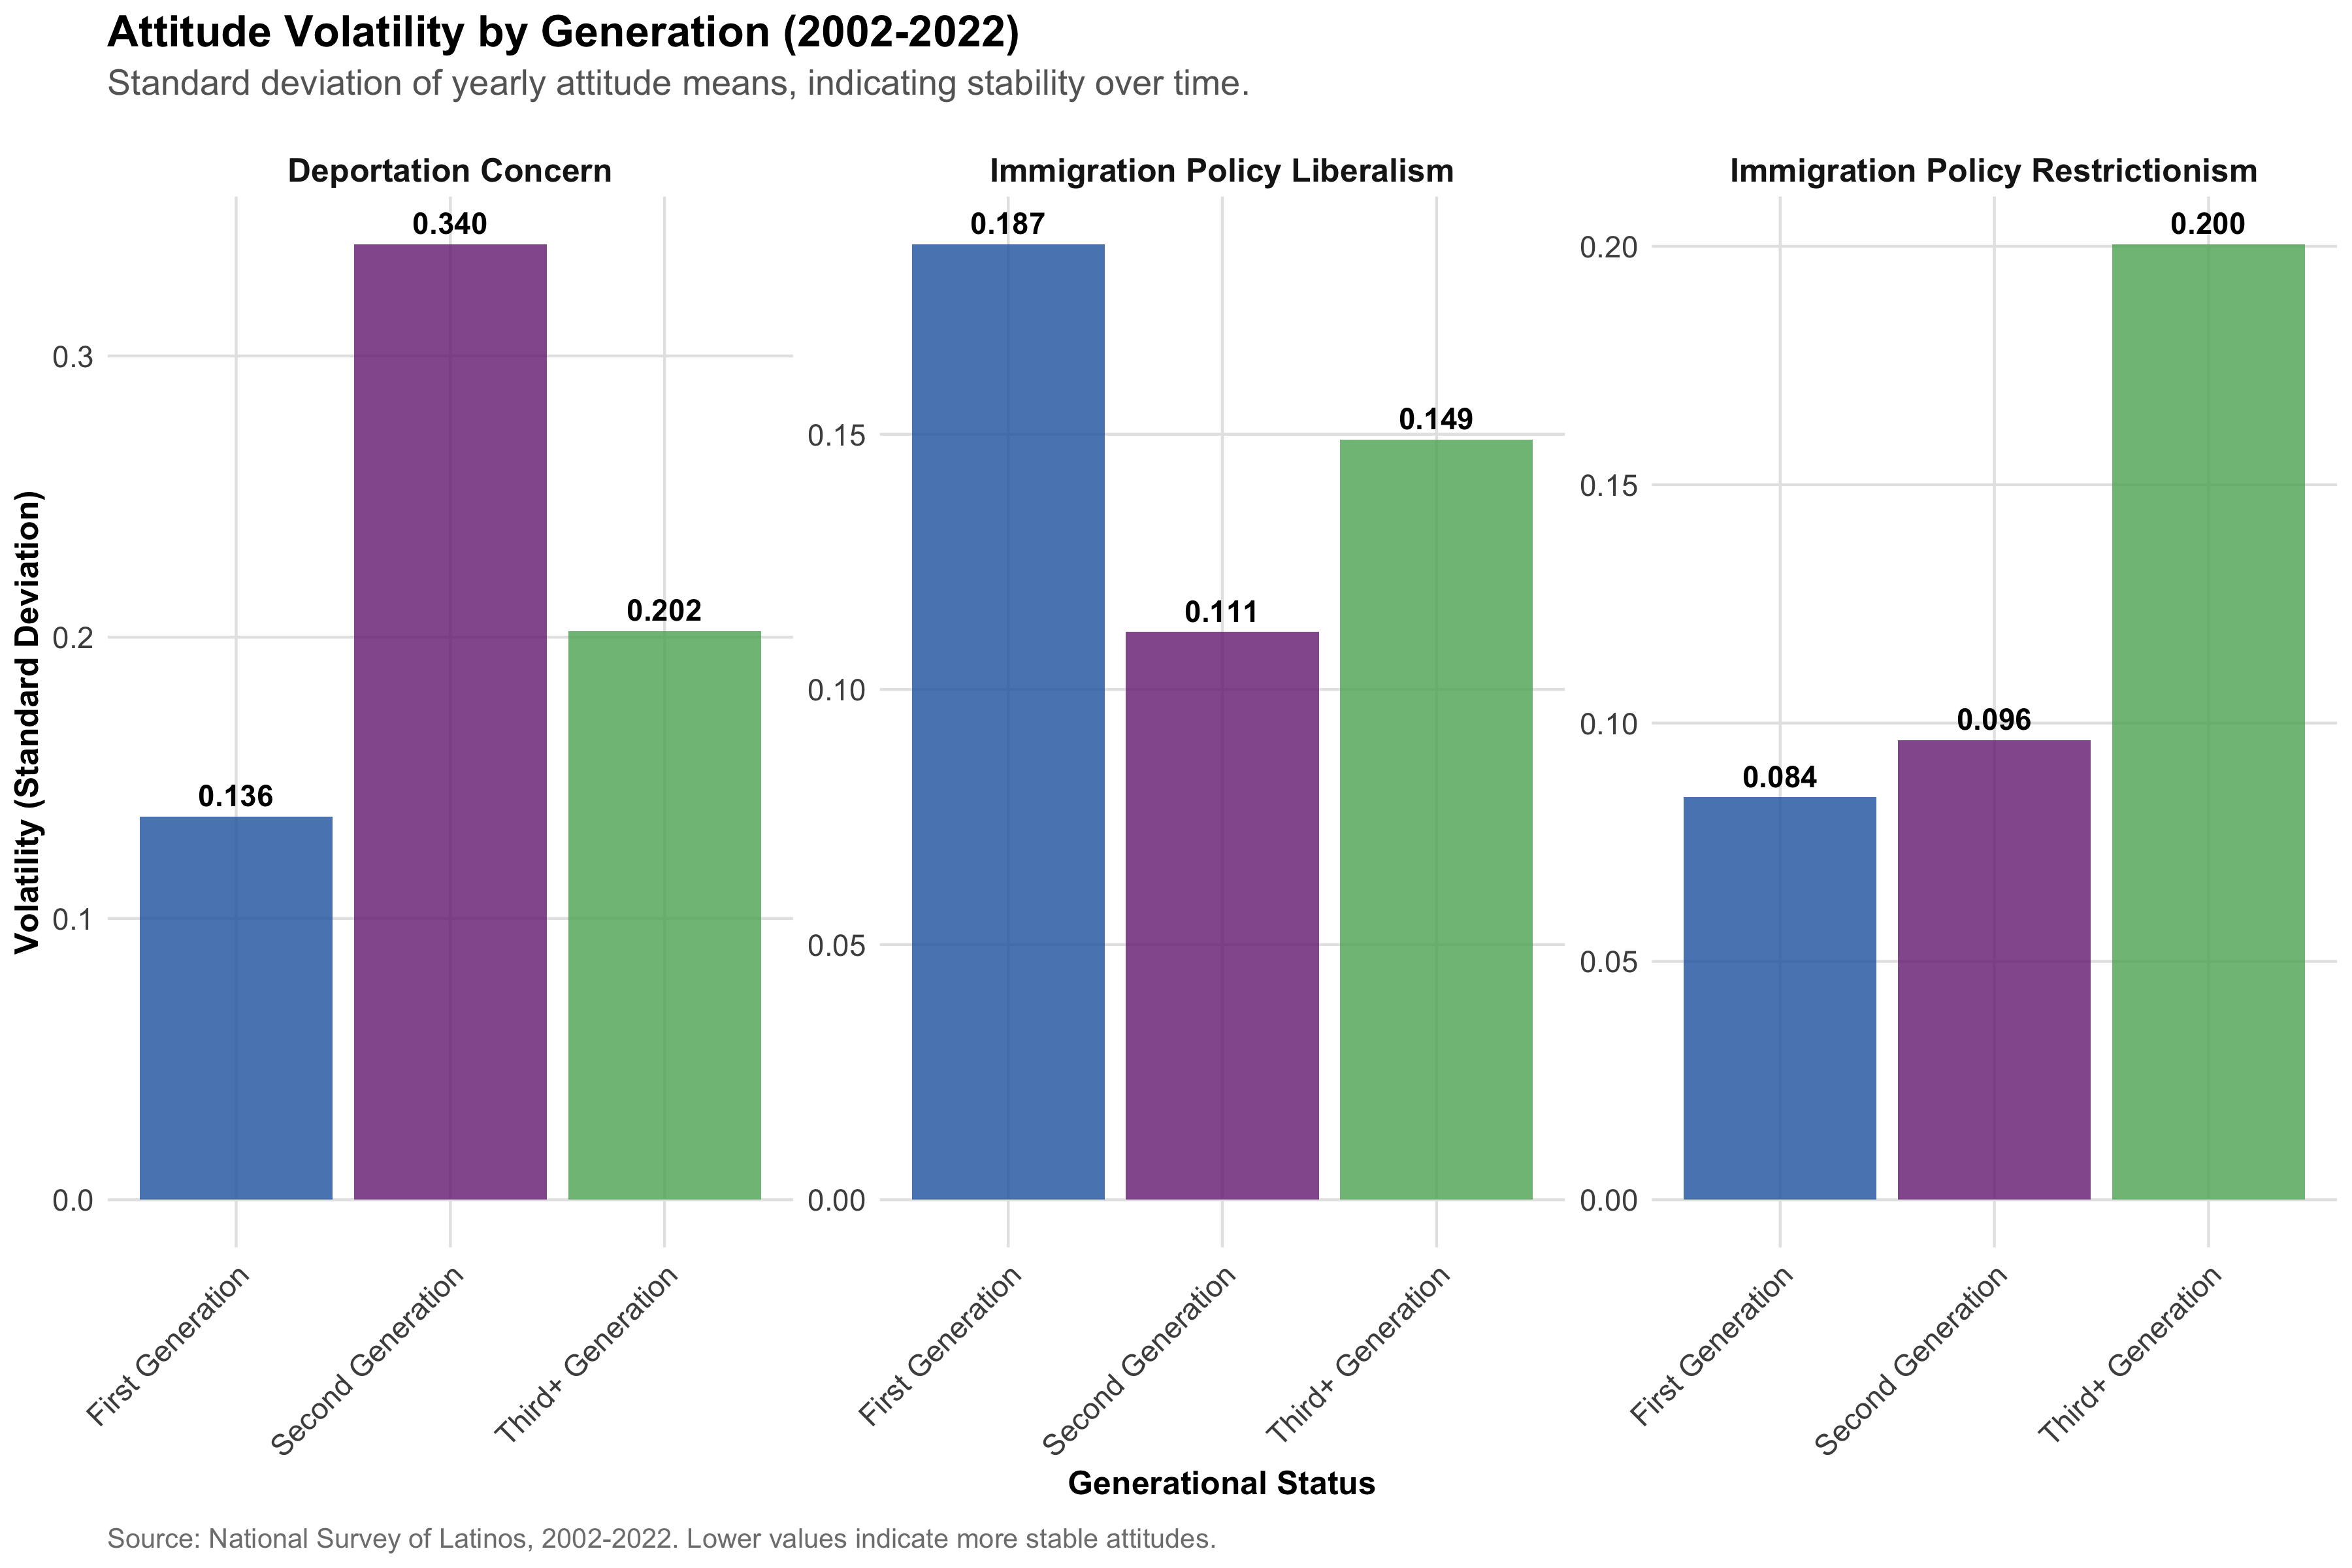
\includegraphics[width=\textwidth]{../../outputs/CURRENT_2025_08_09_FIGURES_gold_standard/volatility_by_generation.png}
    \caption{Attitude volatility by generation, measured as the standard deviation of yearly means. Lower values indicate more stable attitudes over time.}
    \label{fig:volatility}
\end{figure}

\subsection{Statistical Significance}

\begin{figure}[H]
    \centering
    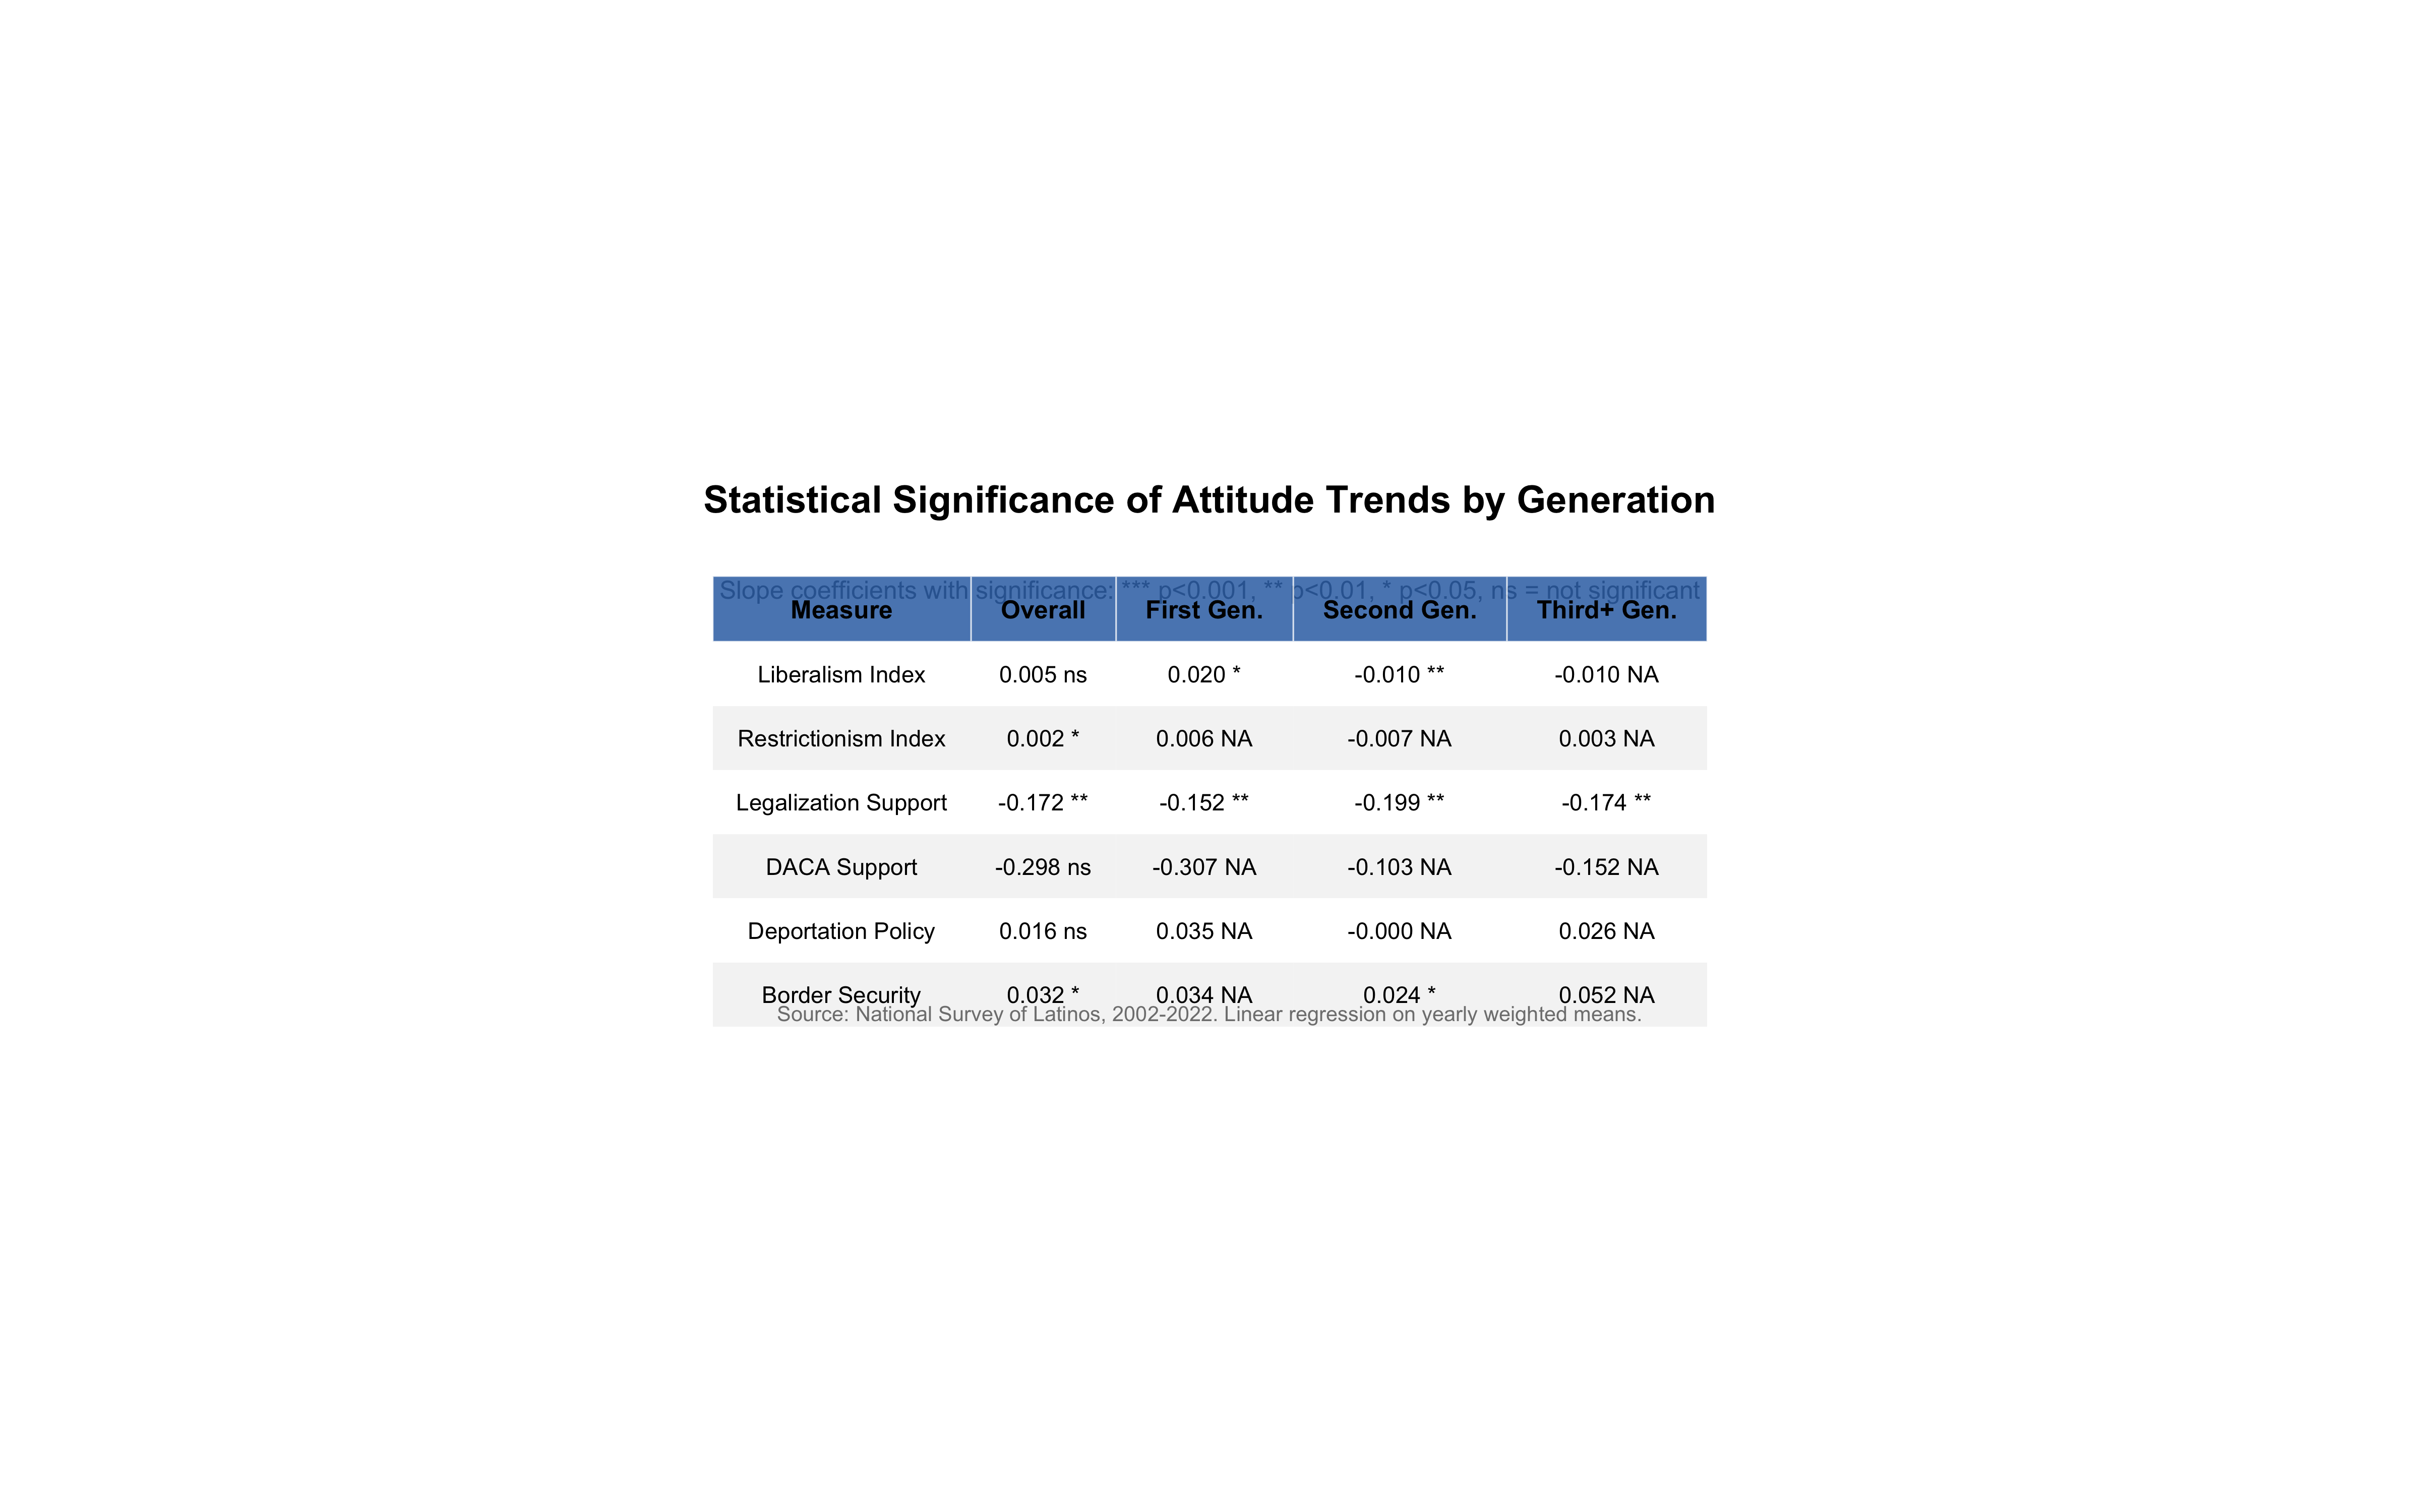
\includegraphics[width=\textwidth]{../../outputs/CURRENT_2025_08_09_FIGURES_gold_standard/significance_table.png}
    \caption{Statistical significance of attitude trends by generation, showing slope coefficients and significance levels from linear regression analyses.}
    \label{fig:significance}
\end{figure}

\subsection{Joinpoint Analysis}

\begin{figure}[H]
    \centering
    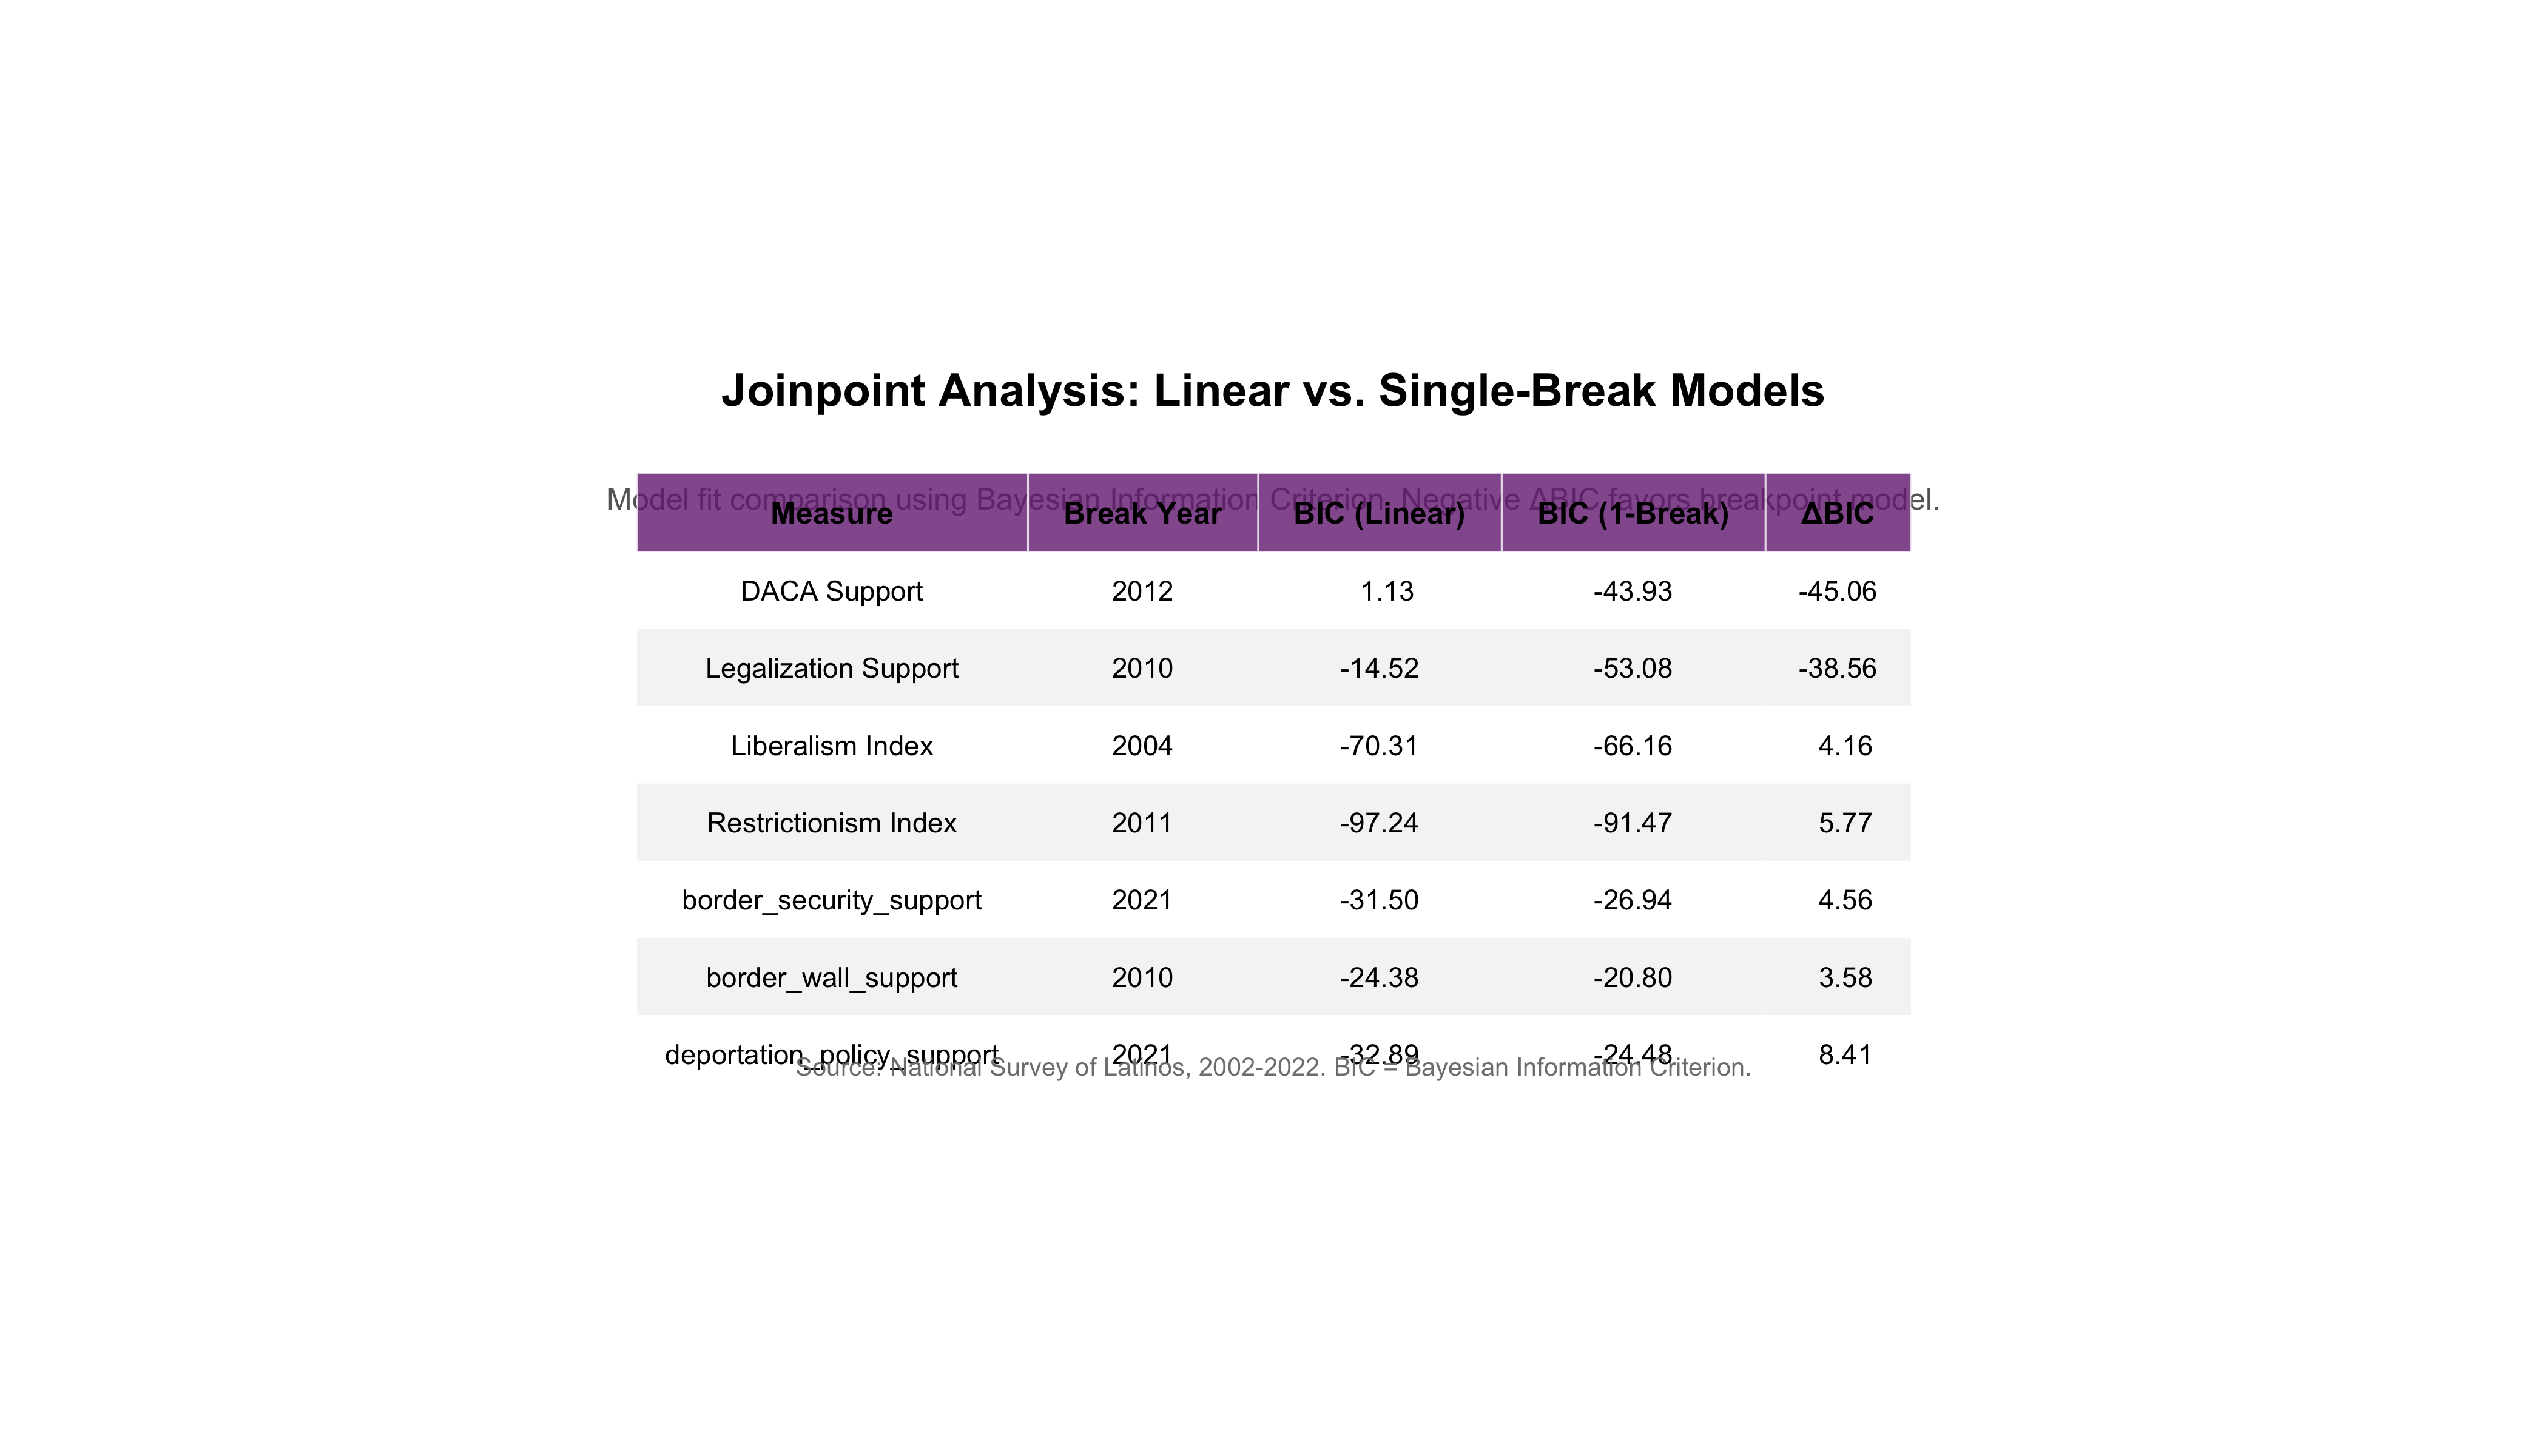
\includegraphics[width=\textwidth]{../../outputs/CURRENT_2025_08_09_FIGURES_gold_standard/joinpoint_analysis_summary.png}
    \caption{Joinpoint analysis comparing linear trends versus single-breakpoint models, with Bayesian Information Criterion values for model comparison.}
    \label{fig:joinpoint}
\end{figure}

\section*{Methodology Note}

All analyses employ weighted OLS regression on yearly means without fixed effects (NOFE approach). Color coding is consistent across all figures: First Generation (blue), Second Generation (purple), Third+ Generation (green). Confidence intervals represent 95\% confidence bounds where shown.

\section*{Data Source}

National Survey of Latinos, 2002-2022. Pew Research Center and various survey organizations. Sample sizes and coverage vary by measure and year as documented in the coverage matrix.

\end{document}
